\documentclass[twoside]{book}

% Packages required by doxygen
\usepackage{fixltx2e}
\usepackage{calc}
\usepackage{doxygen}
\usepackage[export]{adjustbox} % also loads graphicx
\usepackage{graphicx}
\usepackage[utf8]{inputenc}
\usepackage{makeidx}
\usepackage{multicol}
\usepackage{multirow}
\PassOptionsToPackage{warn}{textcomp}
\usepackage{textcomp}
\usepackage[nointegrals]{wasysym}
\usepackage[table]{xcolor}

% Font selection
\usepackage[T1]{fontenc}
\usepackage[scaled=.90]{helvet}
\usepackage{courier}
\usepackage{amssymb}
\usepackage{sectsty}
\renewcommand{\familydefault}{\sfdefault}
\allsectionsfont{%
  \fontseries{bc}\selectfont%
  \color{darkgray}%
}
\renewcommand{\DoxyLabelFont}{%
  \fontseries{bc}\selectfont%
  \color{darkgray}%
}
\newcommand{\+}{\discretionary{\mbox{\scriptsize$\hookleftarrow$}}{}{}}

% Page & text layout
\usepackage{geometry}
\geometry{%
  a4paper,%
  top=2.5cm,%
  bottom=2.5cm,%
  left=2.5cm,%
  right=2.5cm%
}
\tolerance=750
\hfuzz=15pt
\hbadness=750
\setlength{\emergencystretch}{15pt}
\setlength{\parindent}{0cm}
\setlength{\parskip}{3ex plus 2ex minus 2ex}
\makeatletter
\renewcommand{\paragraph}{%
  \@startsection{paragraph}{4}{0ex}{-1.0ex}{1.0ex}{%
    \normalfont\normalsize\bfseries\SS@parafont%
  }%
}
\renewcommand{\subparagraph}{%
  \@startsection{subparagraph}{5}{0ex}{-1.0ex}{1.0ex}{%
    \normalfont\normalsize\bfseries\SS@subparafont%
  }%
}
\makeatother

% Headers & footers
\usepackage{fancyhdr}
\pagestyle{fancyplain}
\fancyhead[LE]{\fancyplain{}{\bfseries\thepage}}
\fancyhead[CE]{\fancyplain{}{}}
\fancyhead[RE]{\fancyplain{}{\bfseries\leftmark}}
\fancyhead[LO]{\fancyplain{}{\bfseries\rightmark}}
\fancyhead[CO]{\fancyplain{}{}}
\fancyhead[RO]{\fancyplain{}{\bfseries\thepage}}
\fancyfoot[LE]{\fancyplain{}{}}
\fancyfoot[CE]{\fancyplain{}{}}
\fancyfoot[RE]{\fancyplain{}{\bfseries\scriptsize Generated by Doxygen }}
\fancyfoot[LO]{\fancyplain{}{\bfseries\scriptsize Generated by Doxygen }}
\fancyfoot[CO]{\fancyplain{}{}}
\fancyfoot[RO]{\fancyplain{}{}}
\renewcommand{\footrulewidth}{0.4pt}
\renewcommand{\chaptermark}[1]{%
  \markboth{#1}{}%
}
\renewcommand{\sectionmark}[1]{%
  \markright{\thesection\ #1}%
}

% Indices & bibliography
\usepackage{natbib}
\usepackage[titles]{tocloft}
\setcounter{tocdepth}{3}
\setcounter{secnumdepth}{5}
\makeindex

% Hyperlinks (required, but should be loaded last)
\usepackage{ifpdf}
\ifpdf
  \usepackage[pdftex,pagebackref=true]{hyperref}
\else
  \usepackage[ps2pdf,pagebackref=true]{hyperref}
\fi
\hypersetup{%
  colorlinks=true,%
  linkcolor=blue,%
  citecolor=blue,%
  unicode%
}

% Custom commands
\newcommand{\clearemptydoublepage}{%
  \newpage{\pagestyle{empty}\cleardoublepage}%
}

\usepackage{caption}
\captionsetup{labelsep=space,justification=centering,font={bf},singlelinecheck=off,skip=4pt,position=top}

%===== C O N T E N T S =====

\begin{document}

% Titlepage & ToC
\hypersetup{pageanchor=false,
             bookmarksnumbered=true,
             pdfencoding=unicode
            }
\pagenumbering{alph}
\begin{titlepage}
\vspace*{7cm}
\begin{center}%
{\Large My Project \\[1ex]\large 1 }\\
\vspace*{1cm}
{\large Generated by Doxygen 1.8.13}\\
\end{center}
\end{titlepage}
\clearemptydoublepage
\pagenumbering{roman}
\tableofcontents
\clearemptydoublepage
\pagenumbering{arabic}
\hypersetup{pageanchor=true}

%--- Begin generated contents ---
\chapter{R\+T\+L-\/\+R\+FM}
\label{md__r_e_a_d_m_e}
\Hypertarget{md__r_e_a_d_m_e}
F\+S\+K/\+G\+F\+SK Decoder for R\+T\+L-\/\+S\+DR

\subsection*{Usage }


\begin{DoxyCode}
RTL\_RFM, (C) Ryan Suchocki

Usage: rtl\_rfm [-hsqd] [-f freq] [-g gain] [-p error] 

Option flags:
  -h    Show this message
  -s    Read input from stdin
  -q    Quiet. Only output good messages
  -d    Show Debug Plot
  -f    Frequency [869412500]
  -g    Gain [50]
  -p    PPM error [47]
\end{DoxyCode}
 
\chapter{File Index}
\section{File List}
Here is a list of all files with brief descriptions\+:\begin{DoxyCompactList}
\item\contentsline{section}{\hyperlink{downsampler_8c}{downsampler.\+c} }{\pageref{downsampler_8c}}{}
\item\contentsline{section}{\hyperlink{downsampler_8h}{downsampler.\+h} }{\pageref{downsampler_8h}}{}
\item\contentsline{section}{\hyperlink{fm_8c}{fm.\+c} }{\pageref{fm_8c}}{}
\item\contentsline{section}{\hyperlink{fm_8h}{fm.\+h} }{\pageref{fm_8h}}{}
\item\contentsline{section}{\hyperlink{fsk_8c}{fsk.\+c} }{\pageref{fsk_8c}}{}
\item\contentsline{section}{\hyperlink{fsk_8h}{fsk.\+h} }{\pageref{fsk_8h}}{}
\item\contentsline{section}{\hyperlink{rfm__protocol_8c}{rfm\+\_\+protocol.\+c} }{\pageref{rfm__protocol_8c}}{}
\item\contentsline{section}{\hyperlink{rfm__protocol_8h}{rfm\+\_\+protocol.\+h} }{\pageref{rfm__protocol_8h}}{}
\item\contentsline{section}{\hyperlink{rtl__rfm_8c}{rtl\+\_\+rfm.\+c} }{\pageref{rtl__rfm_8c}}{}
\item\contentsline{section}{\hyperlink{rtl__rfm_8h}{rtl\+\_\+rfm.\+h} }{\pageref{rtl__rfm_8h}}{}
\end{DoxyCompactList}

\chapter{File Documentation}
\hypertarget{downsampler_8c}{}\section{downsampler.\+c File Reference}
\label{downsampler_8c}\index{downsampler.\+c@{downsampler.\+c}}
{\ttfamily \#include $<$stdio.\+h$>$}\newline
{\ttfamily \#include $<$stdlib.\+h$>$}\newline
{\ttfamily \#include $<$stdbool.\+h$>$}\newline
{\ttfamily \#include $<$stdint.\+h$>$}\newline
{\ttfamily \#include $<$unistd.\+h$>$}\newline
{\ttfamily \#include $<$ctype.\+h$>$}\newline
{\ttfamily \#include $<$string.\+h$>$}\newline
{\ttfamily \#include $<$math.\+h$>$}\newline
{\ttfamily \#include $<$time.\+h$>$}\newline
{\ttfamily \#include \char`\"{}rtl\+\_\+rfm.\+h\char`\"{}}\newline
{\ttfamily \#include \char`\"{}downsampler.\+h\char`\"{}}\newline
Include dependency graph for downsampler.\+c\+:
\nopagebreak
\begin{figure}[H]
\begin{center}
\leavevmode
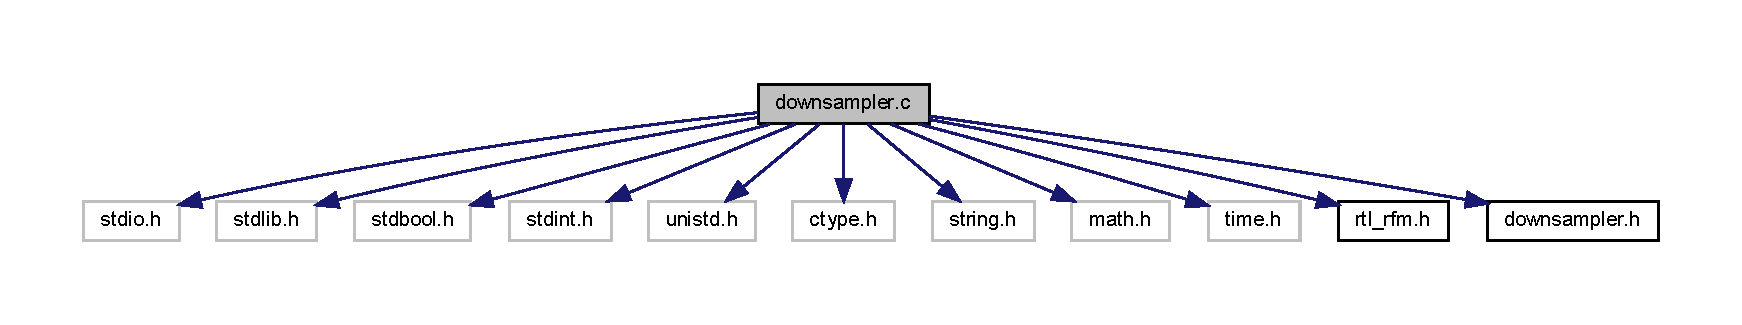
\includegraphics[width=350pt]{downsampler_8c__incl}
\end{center}
\end{figure}
\subsection*{Functions}
\begin{DoxyCompactItemize}
\item 
void \hyperlink{downsampler_8c_abaea1412d36c238f155dada03df2d900}{downsampler\+\_\+init} ()
\item 
bool \hyperlink{downsampler_8c_adf43368ebff559c63105203d3df56e47}{downsampler} (int8\+\_\+t newi, int8\+\_\+t newq)
\item 
int8\+\_\+t \hyperlink{downsampler_8c_a1e27c90a0a81573342ea44e9149d6417}{getI} ()
\item 
int8\+\_\+t \hyperlink{downsampler_8c_a5e89160f5ffae1026c9cc21f4ab2abcc}{getQ} ()
\end{DoxyCompactItemize}
\subsection*{Variables}
\begin{DoxyCompactItemize}
\item 
int8\+\_\+t \hyperlink{downsampler_8c_ad5960b91146cfef0ce43f5787a4c039b}{ibuf} \mbox{[}\hyperlink{rtl__rfm_8h_a061e870517c5d5c01d232d72e5b6857f}{D\+O\+W\+N\+S\+A\+M\+P\+LE}\mbox{]}
\item 
int8\+\_\+t \hyperlink{downsampler_8c_ae4cf2ded73bff3999b19dcded17a2c7d}{qbuf} \mbox{[}\hyperlink{rtl__rfm_8h_a061e870517c5d5c01d232d72e5b6857f}{D\+O\+W\+N\+S\+A\+M\+P\+LE}\mbox{]}
\item 
uint8\+\_\+t \hyperlink{downsampler_8c_a01e8922c4e821da63d9b5060a0a30f45}{bufi} = 0
\item 
int16\+\_\+t \hyperlink{downsampler_8c_acf6c0ad89b09caa5a9458c96bc8b0abb}{icount} = 0
\item 
int16\+\_\+t \hyperlink{downsampler_8c_a6ad9b208c724b45811ffb0742a0251a3}{qcount} = 0
\end{DoxyCompactItemize}


\subsection{Function Documentation}
\mbox{\Hypertarget{downsampler_8c_adf43368ebff559c63105203d3df56e47}\label{downsampler_8c_adf43368ebff559c63105203d3df56e47}} 
\index{downsampler.\+c@{downsampler.\+c}!downsampler@{downsampler}}
\index{downsampler@{downsampler}!downsampler.\+c@{downsampler.\+c}}
\subsubsection{\texorpdfstring{downsampler()}{downsampler()}}
{\footnotesize\ttfamily bool downsampler (\begin{DoxyParamCaption}\item[{int8\+\_\+t}]{newi,  }\item[{int8\+\_\+t}]{newq }\end{DoxyParamCaption})}

\mbox{\Hypertarget{downsampler_8c_abaea1412d36c238f155dada03df2d900}\label{downsampler_8c_abaea1412d36c238f155dada03df2d900}} 
\index{downsampler.\+c@{downsampler.\+c}!downsampler\+\_\+init@{downsampler\+\_\+init}}
\index{downsampler\+\_\+init@{downsampler\+\_\+init}!downsampler.\+c@{downsampler.\+c}}
\subsubsection{\texorpdfstring{downsampler\+\_\+init()}{downsampler\_init()}}
{\footnotesize\ttfamily void downsampler\+\_\+init (\begin{DoxyParamCaption}{ }\end{DoxyParamCaption})}

\mbox{\Hypertarget{downsampler_8c_a1e27c90a0a81573342ea44e9149d6417}\label{downsampler_8c_a1e27c90a0a81573342ea44e9149d6417}} 
\index{downsampler.\+c@{downsampler.\+c}!getI@{getI}}
\index{getI@{getI}!downsampler.\+c@{downsampler.\+c}}
\subsubsection{\texorpdfstring{get\+I()}{getI()}}
{\footnotesize\ttfamily int8\+\_\+t getI (\begin{DoxyParamCaption}{ }\end{DoxyParamCaption})}

\mbox{\Hypertarget{downsampler_8c_a5e89160f5ffae1026c9cc21f4ab2abcc}\label{downsampler_8c_a5e89160f5ffae1026c9cc21f4ab2abcc}} 
\index{downsampler.\+c@{downsampler.\+c}!getQ@{getQ}}
\index{getQ@{getQ}!downsampler.\+c@{downsampler.\+c}}
\subsubsection{\texorpdfstring{get\+Q()}{getQ()}}
{\footnotesize\ttfamily int8\+\_\+t getQ (\begin{DoxyParamCaption}{ }\end{DoxyParamCaption})}



\subsection{Variable Documentation}
\mbox{\Hypertarget{downsampler_8c_a01e8922c4e821da63d9b5060a0a30f45}\label{downsampler_8c_a01e8922c4e821da63d9b5060a0a30f45}} 
\index{downsampler.\+c@{downsampler.\+c}!bufi@{bufi}}
\index{bufi@{bufi}!downsampler.\+c@{downsampler.\+c}}
\subsubsection{\texorpdfstring{bufi}{bufi}}
{\footnotesize\ttfamily uint8\+\_\+t bufi = 0}

\mbox{\Hypertarget{downsampler_8c_ad5960b91146cfef0ce43f5787a4c039b}\label{downsampler_8c_ad5960b91146cfef0ce43f5787a4c039b}} 
\index{downsampler.\+c@{downsampler.\+c}!ibuf@{ibuf}}
\index{ibuf@{ibuf}!downsampler.\+c@{downsampler.\+c}}
\subsubsection{\texorpdfstring{ibuf}{ibuf}}
{\footnotesize\ttfamily int8\+\_\+t ibuf\mbox{[}\hyperlink{rtl__rfm_8h_a061e870517c5d5c01d232d72e5b6857f}{D\+O\+W\+N\+S\+A\+M\+P\+LE}\mbox{]}}

\mbox{\Hypertarget{downsampler_8c_acf6c0ad89b09caa5a9458c96bc8b0abb}\label{downsampler_8c_acf6c0ad89b09caa5a9458c96bc8b0abb}} 
\index{downsampler.\+c@{downsampler.\+c}!icount@{icount}}
\index{icount@{icount}!downsampler.\+c@{downsampler.\+c}}
\subsubsection{\texorpdfstring{icount}{icount}}
{\footnotesize\ttfamily int16\+\_\+t icount = 0}

\mbox{\Hypertarget{downsampler_8c_ae4cf2ded73bff3999b19dcded17a2c7d}\label{downsampler_8c_ae4cf2ded73bff3999b19dcded17a2c7d}} 
\index{downsampler.\+c@{downsampler.\+c}!qbuf@{qbuf}}
\index{qbuf@{qbuf}!downsampler.\+c@{downsampler.\+c}}
\subsubsection{\texorpdfstring{qbuf}{qbuf}}
{\footnotesize\ttfamily int8\+\_\+t qbuf\mbox{[}\hyperlink{rtl__rfm_8h_a061e870517c5d5c01d232d72e5b6857f}{D\+O\+W\+N\+S\+A\+M\+P\+LE}\mbox{]}}

\mbox{\Hypertarget{downsampler_8c_a6ad9b208c724b45811ffb0742a0251a3}\label{downsampler_8c_a6ad9b208c724b45811ffb0742a0251a3}} 
\index{downsampler.\+c@{downsampler.\+c}!qcount@{qcount}}
\index{qcount@{qcount}!downsampler.\+c@{downsampler.\+c}}
\subsubsection{\texorpdfstring{qcount}{qcount}}
{\footnotesize\ttfamily int16\+\_\+t qcount = 0}


\hypertarget{downsampler_8h}{}\section{downsampler.\+h File Reference}
\label{downsampler_8h}\index{downsampler.\+h@{downsampler.\+h}}
This graph shows which files directly or indirectly include this file\+:
\nopagebreak
\begin{figure}[H]
\begin{center}
\leavevmode
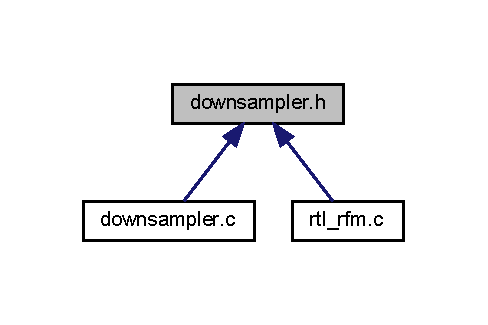
\includegraphics[width=234pt]{downsampler_8h__dep__incl}
\end{center}
\end{figure}
\subsection*{Functions}
\begin{DoxyCompactItemize}
\item 
void \hyperlink{downsampler_8h_abaea1412d36c238f155dada03df2d900}{downsampler\+\_\+init} ()
\item 
bool \hyperlink{downsampler_8h_a7314e94bde4fc108a77d34875c339cd4}{downsampler} (int8\+\_\+t newreal, int8\+\_\+t newimag)
\item 
int8\+\_\+t \hyperlink{downsampler_8h_a1e27c90a0a81573342ea44e9149d6417}{getI} ()
\item 
int8\+\_\+t \hyperlink{downsampler_8h_a5e89160f5ffae1026c9cc21f4ab2abcc}{getQ} ()
\end{DoxyCompactItemize}


\subsection{Function Documentation}
\mbox{\Hypertarget{downsampler_8h_a7314e94bde4fc108a77d34875c339cd4}\label{downsampler_8h_a7314e94bde4fc108a77d34875c339cd4}} 
\index{downsampler.\+h@{downsampler.\+h}!downsampler@{downsampler}}
\index{downsampler@{downsampler}!downsampler.\+h@{downsampler.\+h}}
\subsubsection{\texorpdfstring{downsampler()}{downsampler()}}
{\footnotesize\ttfamily bool downsampler (\begin{DoxyParamCaption}\item[{int8\+\_\+t}]{newreal,  }\item[{int8\+\_\+t}]{newimag }\end{DoxyParamCaption})}

\mbox{\Hypertarget{downsampler_8h_abaea1412d36c238f155dada03df2d900}\label{downsampler_8h_abaea1412d36c238f155dada03df2d900}} 
\index{downsampler.\+h@{downsampler.\+h}!downsampler\+\_\+init@{downsampler\+\_\+init}}
\index{downsampler\+\_\+init@{downsampler\+\_\+init}!downsampler.\+h@{downsampler.\+h}}
\subsubsection{\texorpdfstring{downsampler\+\_\+init()}{downsampler\_init()}}
{\footnotesize\ttfamily void downsampler\+\_\+init (\begin{DoxyParamCaption}{ }\end{DoxyParamCaption})}

\mbox{\Hypertarget{downsampler_8h_a1e27c90a0a81573342ea44e9149d6417}\label{downsampler_8h_a1e27c90a0a81573342ea44e9149d6417}} 
\index{downsampler.\+h@{downsampler.\+h}!getI@{getI}}
\index{getI@{getI}!downsampler.\+h@{downsampler.\+h}}
\subsubsection{\texorpdfstring{get\+I()}{getI()}}
{\footnotesize\ttfamily int8\+\_\+t getI (\begin{DoxyParamCaption}{ }\end{DoxyParamCaption})}

\mbox{\Hypertarget{downsampler_8h_a5e89160f5ffae1026c9cc21f4ab2abcc}\label{downsampler_8h_a5e89160f5ffae1026c9cc21f4ab2abcc}} 
\index{downsampler.\+h@{downsampler.\+h}!getQ@{getQ}}
\index{getQ@{getQ}!downsampler.\+h@{downsampler.\+h}}
\subsubsection{\texorpdfstring{get\+Q()}{getQ()}}
{\footnotesize\ttfamily int8\+\_\+t getQ (\begin{DoxyParamCaption}{ }\end{DoxyParamCaption})}


\hypertarget{fm_8c}{}\section{fm.\+c File Reference}
\label{fm_8c}\index{fm.\+c@{fm.\+c}}
{\ttfamily \#include $<$stdio.\+h$>$}\newline
{\ttfamily \#include $<$stdlib.\+h$>$}\newline
{\ttfamily \#include $<$stdbool.\+h$>$}\newline
{\ttfamily \#include $<$stdint.\+h$>$}\newline
{\ttfamily \#include $<$unistd.\+h$>$}\newline
{\ttfamily \#include $<$ctype.\+h$>$}\newline
{\ttfamily \#include $<$string.\+h$>$}\newline
{\ttfamily \#include $<$math.\+h$>$}\newline
{\ttfamily \#include $<$time.\+h$>$}\newline
{\ttfamily \#include \char`\"{}rtl\+\_\+rfm.\+h\char`\"{}}\newline
{\ttfamily \#include \char`\"{}fm.\+h\char`\"{}}\newline
Include dependency graph for fm.\+c\+:
\nopagebreak
\begin{figure}[H]
\begin{center}
\leavevmode
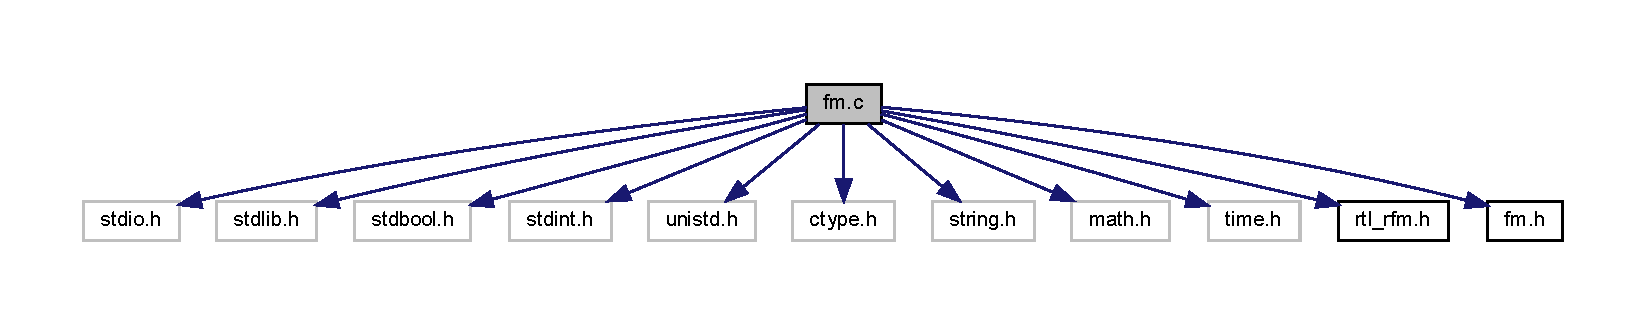
\includegraphics[width=350pt]{fm_8c__incl}
\end{center}
\end{figure}
\subsection*{Macros}
\begin{DoxyCompactItemize}
\item 
\#define \hyperlink{fm_8c_a3d8c9c145887af5174ba4cc6789862ad}{T\+AU}~I\+N\+T16\+\_\+\+M\+AX $\ast$ 2
\item 
\#define \hyperlink{fm_8c_a2bb4bf801d932d9c1abfb3eb22568112}{T\+U\+R\+N\+\_\+1\+\_\+8\+TH}~\hyperlink{fm_8c_a3d8c9c145887af5174ba4cc6789862ad}{T\+AU}$\ast$1/8
\item 
\#define \hyperlink{fm_8c_aaf6ef7b8ff8dce605b8cfa9c8364bd36}{T\+U\+R\+N\+\_\+3\+\_\+8\+TH}~\hyperlink{fm_8c_a3d8c9c145887af5174ba4cc6789862ad}{T\+AU}$\ast$3/8
\item 
\#define \hyperlink{fm_8c_a9b80450b799ce7457386a4176d61d429}{T\+U\+R\+N\+\_\+5\+\_\+8\+TH}~\hyperlink{fm_8c_a3d8c9c145887af5174ba4cc6789862ad}{T\+AU}$\ast$-\/3/8
\item 
\#define \hyperlink{fm_8c_a306872a49dcf2e8b8f980dc9cc5ef6c0}{T\+U\+R\+N\+\_\+7\+\_\+8\+TH}~\hyperlink{fm_8c_a3d8c9c145887af5174ba4cc6789862ad}{T\+AU}$\ast$-\/1/8
\end{DoxyCompactItemize}
\subsection*{Functions}
\begin{DoxyCompactItemize}
\item 
int16\+\_\+t \hyperlink{fm_8c_a84e4162b6361572ff14c221b2ecd1886}{fm\+\_\+demod} (int8\+\_\+t i, int8\+\_\+t q)
\end{DoxyCompactItemize}
\subsection*{Variables}
\begin{DoxyCompactItemize}
\item 
int8\+\_\+t \hyperlink{fm_8c_a495d4a5d22b07efcdaf40bc773c7301b}{pi} = 0
\item 
int8\+\_\+t \hyperlink{fm_8c_ad01c40c0ef89475a2f7a61a91faa8062}{pq} = 0
\item 
int16\+\_\+t \hyperlink{fm_8c_a5087f687dfd18738aff30ce627cc1caa}{fm\+\_\+magnitude} = 0
\end{DoxyCompactItemize}


\subsection{Macro Definition Documentation}
\mbox{\Hypertarget{fm_8c_a3d8c9c145887af5174ba4cc6789862ad}\label{fm_8c_a3d8c9c145887af5174ba4cc6789862ad}} 
\index{fm.\+c@{fm.\+c}!T\+AU@{T\+AU}}
\index{T\+AU@{T\+AU}!fm.\+c@{fm.\+c}}
\subsubsection{\texorpdfstring{T\+AU}{TAU}}
{\footnotesize\ttfamily \#define T\+AU~I\+N\+T16\+\_\+\+M\+AX $\ast$ 2}

\mbox{\Hypertarget{fm_8c_a2bb4bf801d932d9c1abfb3eb22568112}\label{fm_8c_a2bb4bf801d932d9c1abfb3eb22568112}} 
\index{fm.\+c@{fm.\+c}!T\+U\+R\+N\+\_\+1\+\_\+8\+TH@{T\+U\+R\+N\+\_\+1\+\_\+8\+TH}}
\index{T\+U\+R\+N\+\_\+1\+\_\+8\+TH@{T\+U\+R\+N\+\_\+1\+\_\+8\+TH}!fm.\+c@{fm.\+c}}
\subsubsection{\texorpdfstring{T\+U\+R\+N\+\_\+1\+\_\+8\+TH}{TURN\_1\_8TH}}
{\footnotesize\ttfamily \#define T\+U\+R\+N\+\_\+1\+\_\+8\+TH~\hyperlink{fm_8c_a3d8c9c145887af5174ba4cc6789862ad}{T\+AU}$\ast$1/8}

\mbox{\Hypertarget{fm_8c_aaf6ef7b8ff8dce605b8cfa9c8364bd36}\label{fm_8c_aaf6ef7b8ff8dce605b8cfa9c8364bd36}} 
\index{fm.\+c@{fm.\+c}!T\+U\+R\+N\+\_\+3\+\_\+8\+TH@{T\+U\+R\+N\+\_\+3\+\_\+8\+TH}}
\index{T\+U\+R\+N\+\_\+3\+\_\+8\+TH@{T\+U\+R\+N\+\_\+3\+\_\+8\+TH}!fm.\+c@{fm.\+c}}
\subsubsection{\texorpdfstring{T\+U\+R\+N\+\_\+3\+\_\+8\+TH}{TURN\_3\_8TH}}
{\footnotesize\ttfamily \#define T\+U\+R\+N\+\_\+3\+\_\+8\+TH~\hyperlink{fm_8c_a3d8c9c145887af5174ba4cc6789862ad}{T\+AU}$\ast$3/8}

\mbox{\Hypertarget{fm_8c_a9b80450b799ce7457386a4176d61d429}\label{fm_8c_a9b80450b799ce7457386a4176d61d429}} 
\index{fm.\+c@{fm.\+c}!T\+U\+R\+N\+\_\+5\+\_\+8\+TH@{T\+U\+R\+N\+\_\+5\+\_\+8\+TH}}
\index{T\+U\+R\+N\+\_\+5\+\_\+8\+TH@{T\+U\+R\+N\+\_\+5\+\_\+8\+TH}!fm.\+c@{fm.\+c}}
\subsubsection{\texorpdfstring{T\+U\+R\+N\+\_\+5\+\_\+8\+TH}{TURN\_5\_8TH}}
{\footnotesize\ttfamily \#define T\+U\+R\+N\+\_\+5\+\_\+8\+TH~\hyperlink{fm_8c_a3d8c9c145887af5174ba4cc6789862ad}{T\+AU}$\ast$-\/3/8}

\mbox{\Hypertarget{fm_8c_a306872a49dcf2e8b8f980dc9cc5ef6c0}\label{fm_8c_a306872a49dcf2e8b8f980dc9cc5ef6c0}} 
\index{fm.\+c@{fm.\+c}!T\+U\+R\+N\+\_\+7\+\_\+8\+TH@{T\+U\+R\+N\+\_\+7\+\_\+8\+TH}}
\index{T\+U\+R\+N\+\_\+7\+\_\+8\+TH@{T\+U\+R\+N\+\_\+7\+\_\+8\+TH}!fm.\+c@{fm.\+c}}
\subsubsection{\texorpdfstring{T\+U\+R\+N\+\_\+7\+\_\+8\+TH}{TURN\_7\_8TH}}
{\footnotesize\ttfamily \#define T\+U\+R\+N\+\_\+7\+\_\+8\+TH~\hyperlink{fm_8c_a3d8c9c145887af5174ba4cc6789862ad}{T\+AU}$\ast$-\/1/8}



\subsection{Function Documentation}
\mbox{\Hypertarget{fm_8c_a84e4162b6361572ff14c221b2ecd1886}\label{fm_8c_a84e4162b6361572ff14c221b2ecd1886}} 
\index{fm.\+c@{fm.\+c}!fm\+\_\+demod@{fm\+\_\+demod}}
\index{fm\+\_\+demod@{fm\+\_\+demod}!fm.\+c@{fm.\+c}}
\subsubsection{\texorpdfstring{fm\+\_\+demod()}{fm\_demod()}}
{\footnotesize\ttfamily int16\+\_\+t fm\+\_\+demod (\begin{DoxyParamCaption}\item[{int8\+\_\+t}]{i,  }\item[{int8\+\_\+t}]{q }\end{DoxyParamCaption})}



\subsection{Variable Documentation}
\mbox{\Hypertarget{fm_8c_a5087f687dfd18738aff30ce627cc1caa}\label{fm_8c_a5087f687dfd18738aff30ce627cc1caa}} 
\index{fm.\+c@{fm.\+c}!fm\+\_\+magnitude@{fm\+\_\+magnitude}}
\index{fm\+\_\+magnitude@{fm\+\_\+magnitude}!fm.\+c@{fm.\+c}}
\subsubsection{\texorpdfstring{fm\+\_\+magnitude}{fm\_magnitude}}
{\footnotesize\ttfamily int16\+\_\+t fm\+\_\+magnitude = 0}

\mbox{\Hypertarget{fm_8c_a495d4a5d22b07efcdaf40bc773c7301b}\label{fm_8c_a495d4a5d22b07efcdaf40bc773c7301b}} 
\index{fm.\+c@{fm.\+c}!pi@{pi}}
\index{pi@{pi}!fm.\+c@{fm.\+c}}
\subsubsection{\texorpdfstring{pi}{pi}}
{\footnotesize\ttfamily int8\+\_\+t pi = 0}

\mbox{\Hypertarget{fm_8c_ad01c40c0ef89475a2f7a61a91faa8062}\label{fm_8c_ad01c40c0ef89475a2f7a61a91faa8062}} 
\index{fm.\+c@{fm.\+c}!pq@{pq}}
\index{pq@{pq}!fm.\+c@{fm.\+c}}
\subsubsection{\texorpdfstring{pq}{pq}}
{\footnotesize\ttfamily int8\+\_\+t pq = 0}


\hypertarget{fm_8h}{}\section{fm.\+h File Reference}
\label{fm_8h}\index{fm.\+h@{fm.\+h}}
This graph shows which files directly or indirectly include this file\+:
\nopagebreak
\begin{figure}[H]
\begin{center}
\leavevmode
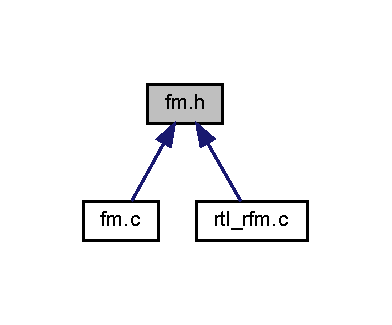
\includegraphics[width=188pt]{fm_8h__dep__incl}
\end{center}
\end{figure}
\subsection*{Functions}
\begin{DoxyCompactItemize}
\item 
int16\+\_\+t \hyperlink{fm_8h_ab05cb69cae73a3fe6c19de8a45cfde90}{fm\+\_\+demod} (int8\+\_\+t real, int8\+\_\+t imag)
\end{DoxyCompactItemize}
\subsection*{Variables}
\begin{DoxyCompactItemize}
\item 
int16\+\_\+t \hyperlink{fm_8h_a5087f687dfd18738aff30ce627cc1caa}{fm\+\_\+magnitude}
\end{DoxyCompactItemize}


\subsection{Function Documentation}
\mbox{\Hypertarget{fm_8h_ab05cb69cae73a3fe6c19de8a45cfde90}\label{fm_8h_ab05cb69cae73a3fe6c19de8a45cfde90}} 
\index{fm.\+h@{fm.\+h}!fm\+\_\+demod@{fm\+\_\+demod}}
\index{fm\+\_\+demod@{fm\+\_\+demod}!fm.\+h@{fm.\+h}}
\subsubsection{\texorpdfstring{fm\+\_\+demod()}{fm\_demod()}}
{\footnotesize\ttfamily int16\+\_\+t fm\+\_\+demod (\begin{DoxyParamCaption}\item[{int8\+\_\+t}]{real,  }\item[{int8\+\_\+t}]{imag }\end{DoxyParamCaption})}



\subsection{Variable Documentation}
\mbox{\Hypertarget{fm_8h_a5087f687dfd18738aff30ce627cc1caa}\label{fm_8h_a5087f687dfd18738aff30ce627cc1caa}} 
\index{fm.\+h@{fm.\+h}!fm\+\_\+magnitude@{fm\+\_\+magnitude}}
\index{fm\+\_\+magnitude@{fm\+\_\+magnitude}!fm.\+h@{fm.\+h}}
\subsubsection{\texorpdfstring{fm\+\_\+magnitude}{fm\_magnitude}}
{\footnotesize\ttfamily int16\+\_\+t fm\+\_\+magnitude}


\hypertarget{fsk_8c}{}\section{fsk.\+c File Reference}
\label{fsk_8c}\index{fsk.\+c@{fsk.\+c}}
{\ttfamily \#include $<$stdio.\+h$>$}\newline
{\ttfamily \#include $<$stdlib.\+h$>$}\newline
{\ttfamily \#include $<$stdbool.\+h$>$}\newline
{\ttfamily \#include $<$stdint.\+h$>$}\newline
{\ttfamily \#include $<$unistd.\+h$>$}\newline
{\ttfamily \#include $<$ctype.\+h$>$}\newline
{\ttfamily \#include $<$string.\+h$>$}\newline
{\ttfamily \#include $<$math.\+h$>$}\newline
{\ttfamily \#include $<$time.\+h$>$}\newline
{\ttfamily \#include \char`\"{}rtl\+\_\+rfm.\+h\char`\"{}}\newline
{\ttfamily \#include \char`\"{}fsk.\+h\char`\"{}}\newline
Include dependency graph for fsk.\+c\+:
\nopagebreak
\begin{figure}[H]
\begin{center}
\leavevmode
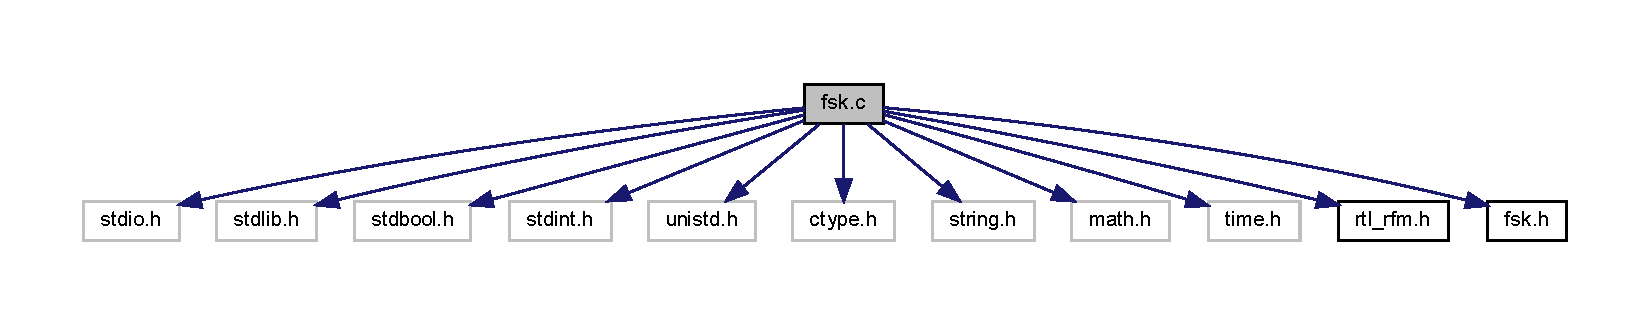
\includegraphics[width=350pt]{fsk_8c__incl}
\end{center}
\end{figure}
\subsection*{Macros}
\begin{DoxyCompactItemize}
\item 
\#define \hyperlink{fsk_8c_ab6ba33ac9652520615d41fda4cdc22a4}{C\+L\+K\+P\+E\+R\+I\+OD}~\hyperlink{fsk_8c_a62d68269b9adfd52e062cf0a26b964b5}{windowsize}
\end{DoxyCompactItemize}
\subsection*{Functions}
\begin{DoxyCompactItemize}
\item 
void \hyperlink{fsk_8c_aa5c999a903f4a49095c0acde738ef14e}{fsk\+\_\+init} ()
\item 
void \hyperlink{fsk_8c_a5fc97bcfbea6197fa10974f42cade42c}{fsk\+\_\+cleanup} ()
\item 
int16\+\_\+t \hyperlink{fsk_8c_a3ae4b361fb020e5c152921efa68cc773}{hipass} (int16\+\_\+t sample)
\item 
int16\+\_\+t \hyperlink{fsk_8c_ae92e6569cac83fcd4a1f7f8345141a37}{lopass} (int16\+\_\+t sample)
\item 
int32\+\_\+t \hyperlink{fsk_8c_a6065e8cc94d4facccb1504c526ef9249}{moving\+\_\+average} (int16\+\_\+t sample)
\item 
void \hyperlink{fsk_8c_a26722c58eb057975ec2d15512f42617a}{print\+\_\+waveform} (int16\+\_\+t sample, int16\+\_\+t magnitude)
\item 
int8\+\_\+t \hyperlink{fsk_8c_a7bb9ea952766092f06987bb89d13c60a}{fsk\+\_\+decode} (int16\+\_\+t sample, int16\+\_\+t magnitude)
\end{DoxyCompactItemize}
\subsection*{Variables}
\begin{DoxyCompactItemize}
\item 
int \hyperlink{fsk_8c_ac38751c7169cfeb9325a947cc0484286}{samplerate} = \hyperlink{rtl__rfm_8h_a81ab58068676f17bd9788a2e01dac6d3}{B\+I\+G\+S\+A\+M\+P\+L\+E\+R\+A\+TE}/\hyperlink{rtl__rfm_8h_a061e870517c5d5c01d232d72e5b6857f}{D\+O\+W\+N\+S\+A\+M\+P\+LE}
\item 
int \hyperlink{fsk_8c_a62d68269b9adfd52e062cf0a26b964b5}{windowsize}
\item 
float \hyperlink{fsk_8c_aa7e91fb4ae3d43a619ae7d427767b97e}{fc}
\item 
float \hyperlink{fsk_8c_ac6eeb1cbe583af9fe5192b22f711c34e}{fc2}
\item 
int \hyperlink{fsk_8c_abcaf1ecf494e0f424c115baf97b10cf7}{filtersize}
\item 
int \hyperlink{fsk_8c_afbdcf382ac17287e96101127f2809f13}{filter2size}
\item 
int16\+\_\+t $\ast$ \hyperlink{fsk_8c_af11227c34aa6b7a1a86c52c70f3ac42c}{filter}
\item 
int16\+\_\+t $\ast$ \hyperlink{fsk_8c_a9014a5428cacb3bfcf4ef526f0500827}{filter2}
\item 
int16\+\_\+t $\ast$ \hyperlink{fsk_8c_a803e446eb8281e01816393a233a17972}{mavgbuffer}
\item 
int32\+\_\+t \hyperlink{fsk_8c_a1ef9ae7ff0eb1861a90f8a8018cbd60a}{mavg}
\item 
int \hyperlink{fsk_8c_abc8a6399186a2b36969c3794139afaad}{fi} = 0
\item 
int32\+\_\+t \hyperlink{fsk_8c_a4858b400f708a13bd514376ab941b27d}{count} = 0
\item 
int16\+\_\+t \hyperlink{fsk_8c_a07ad0fc8154b9241a95d8f6bc0241412}{latestoffset} = 0
\item 
int16\+\_\+t \hyperlink{fsk_8c_a466ad671826b40065c323e1f477d5f2d}{offsethold} = 0
\item 
bool \hyperlink{fsk_8c_af0129e079b57e897edf00f22cc25f3d4}{hold} = false
\item 
int \hyperlink{fsk_8c_ad9e97e8c6aafa4f42b57764b699e0dbd}{f2i} = 0
\item 
int32\+\_\+t \hyperlink{fsk_8c_a438dc6eac88a2ca9fb56f24d12ee6232}{count2} = 0
\item 
short \hyperlink{fsk_8c_ace1b45c014904faf7491c708083482d2}{bi} = 0
\item 
int32\+\_\+t \hyperlink{fsk_8c_acd873858ca32196889fa0ceaf480ce64}{mavgcount} = 0
\item 
int \hyperlink{fsk_8c_a78f7c3cc11ce30f992647a9dd42d96eb}{clk} = 1
\item 
int16\+\_\+t \hyperlink{fsk_8c_adeb0c978ff5bc64b2fb5afd41af27a83}{thissample} = 0
\item 
int16\+\_\+t \hyperlink{fsk_8c_a5355441fb9c5428332d6cc7ec4b5f6ad}{prevsample} = 0
\end{DoxyCompactItemize}


\subsection{Macro Definition Documentation}
\mbox{\Hypertarget{fsk_8c_ab6ba33ac9652520615d41fda4cdc22a4}\label{fsk_8c_ab6ba33ac9652520615d41fda4cdc22a4}} 
\index{fsk.\+c@{fsk.\+c}!C\+L\+K\+P\+E\+R\+I\+OD@{C\+L\+K\+P\+E\+R\+I\+OD}}
\index{C\+L\+K\+P\+E\+R\+I\+OD@{C\+L\+K\+P\+E\+R\+I\+OD}!fsk.\+c@{fsk.\+c}}
\subsubsection{\texorpdfstring{C\+L\+K\+P\+E\+R\+I\+OD}{CLKPERIOD}}
{\footnotesize\ttfamily \#define C\+L\+K\+P\+E\+R\+I\+OD~\hyperlink{fsk_8c_a62d68269b9adfd52e062cf0a26b964b5}{windowsize}}



\subsection{Function Documentation}
\mbox{\Hypertarget{fsk_8c_a5fc97bcfbea6197fa10974f42cade42c}\label{fsk_8c_a5fc97bcfbea6197fa10974f42cade42c}} 
\index{fsk.\+c@{fsk.\+c}!fsk\+\_\+cleanup@{fsk\+\_\+cleanup}}
\index{fsk\+\_\+cleanup@{fsk\+\_\+cleanup}!fsk.\+c@{fsk.\+c}}
\subsubsection{\texorpdfstring{fsk\+\_\+cleanup()}{fsk\_cleanup()}}
{\footnotesize\ttfamily void fsk\+\_\+cleanup (\begin{DoxyParamCaption}{ }\end{DoxyParamCaption})}

\mbox{\Hypertarget{fsk_8c_a7bb9ea952766092f06987bb89d13c60a}\label{fsk_8c_a7bb9ea952766092f06987bb89d13c60a}} 
\index{fsk.\+c@{fsk.\+c}!fsk\+\_\+decode@{fsk\+\_\+decode}}
\index{fsk\+\_\+decode@{fsk\+\_\+decode}!fsk.\+c@{fsk.\+c}}
\subsubsection{\texorpdfstring{fsk\+\_\+decode()}{fsk\_decode()}}
{\footnotesize\ttfamily int8\+\_\+t fsk\+\_\+decode (\begin{DoxyParamCaption}\item[{int16\+\_\+t}]{sample,  }\item[{int16\+\_\+t}]{magnitude }\end{DoxyParamCaption})}

Here is the call graph for this function\+:
\nopagebreak
\begin{figure}[H]
\begin{center}
\leavevmode
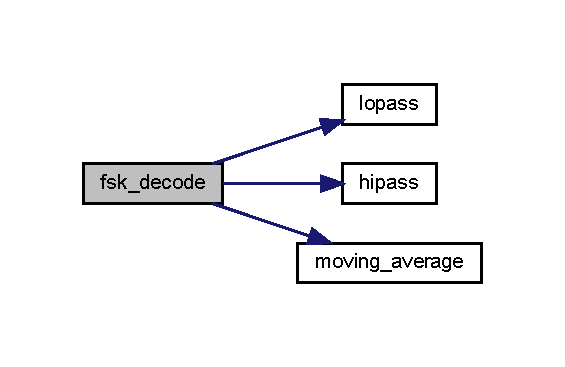
\includegraphics[width=271pt]{fsk_8c_a7bb9ea952766092f06987bb89d13c60a_cgraph}
\end{center}
\end{figure}
\mbox{\Hypertarget{fsk_8c_aa5c999a903f4a49095c0acde738ef14e}\label{fsk_8c_aa5c999a903f4a49095c0acde738ef14e}} 
\index{fsk.\+c@{fsk.\+c}!fsk\+\_\+init@{fsk\+\_\+init}}
\index{fsk\+\_\+init@{fsk\+\_\+init}!fsk.\+c@{fsk.\+c}}
\subsubsection{\texorpdfstring{fsk\+\_\+init()}{fsk\_init()}}
{\footnotesize\ttfamily void fsk\+\_\+init (\begin{DoxyParamCaption}{ }\end{DoxyParamCaption})}

1.\+5; Here is the caller graph for this function\+:
\nopagebreak
\begin{figure}[H]
\begin{center}
\leavevmode
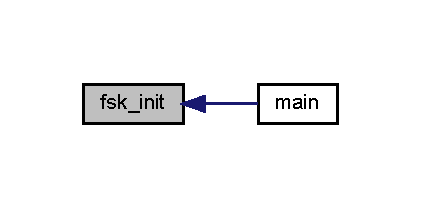
\includegraphics[width=202pt]{fsk_8c_aa5c999a903f4a49095c0acde738ef14e_icgraph}
\end{center}
\end{figure}
\mbox{\Hypertarget{fsk_8c_a3ae4b361fb020e5c152921efa68cc773}\label{fsk_8c_a3ae4b361fb020e5c152921efa68cc773}} 
\index{fsk.\+c@{fsk.\+c}!hipass@{hipass}}
\index{hipass@{hipass}!fsk.\+c@{fsk.\+c}}
\subsubsection{\texorpdfstring{hipass()}{hipass()}}
{\footnotesize\ttfamily int16\+\_\+t hipass (\begin{DoxyParamCaption}\item[{int16\+\_\+t}]{sample }\end{DoxyParamCaption})}

Here is the caller graph for this function\+:
\nopagebreak
\begin{figure}[H]
\begin{center}
\leavevmode
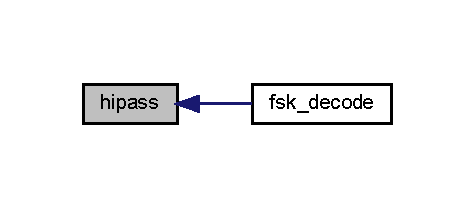
\includegraphics[width=228pt]{fsk_8c_a3ae4b361fb020e5c152921efa68cc773_icgraph}
\end{center}
\end{figure}
\mbox{\Hypertarget{fsk_8c_ae92e6569cac83fcd4a1f7f8345141a37}\label{fsk_8c_ae92e6569cac83fcd4a1f7f8345141a37}} 
\index{fsk.\+c@{fsk.\+c}!lopass@{lopass}}
\index{lopass@{lopass}!fsk.\+c@{fsk.\+c}}
\subsubsection{\texorpdfstring{lopass()}{lopass()}}
{\footnotesize\ttfamily int16\+\_\+t lopass (\begin{DoxyParamCaption}\item[{int16\+\_\+t}]{sample }\end{DoxyParamCaption})}

Here is the caller graph for this function\+:
\nopagebreak
\begin{figure}[H]
\begin{center}
\leavevmode
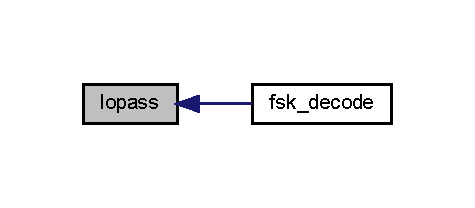
\includegraphics[width=228pt]{fsk_8c_ae92e6569cac83fcd4a1f7f8345141a37_icgraph}
\end{center}
\end{figure}
\mbox{\Hypertarget{fsk_8c_a6065e8cc94d4facccb1504c526ef9249}\label{fsk_8c_a6065e8cc94d4facccb1504c526ef9249}} 
\index{fsk.\+c@{fsk.\+c}!moving\+\_\+average@{moving\+\_\+average}}
\index{moving\+\_\+average@{moving\+\_\+average}!fsk.\+c@{fsk.\+c}}
\subsubsection{\texorpdfstring{moving\+\_\+average()}{moving\_average()}}
{\footnotesize\ttfamily int32\+\_\+t moving\+\_\+average (\begin{DoxyParamCaption}\item[{int16\+\_\+t}]{sample }\end{DoxyParamCaption})}

Here is the caller graph for this function\+:
\nopagebreak
\begin{figure}[H]
\begin{center}
\leavevmode
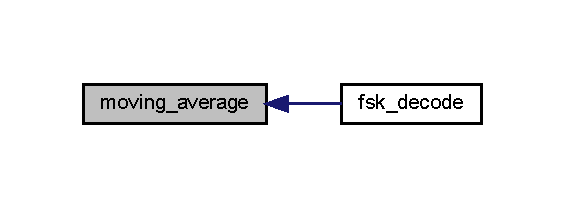
\includegraphics[width=271pt]{fsk_8c_a6065e8cc94d4facccb1504c526ef9249_icgraph}
\end{center}
\end{figure}
\mbox{\Hypertarget{fsk_8c_a26722c58eb057975ec2d15512f42617a}\label{fsk_8c_a26722c58eb057975ec2d15512f42617a}} 
\index{fsk.\+c@{fsk.\+c}!print\+\_\+waveform@{print\+\_\+waveform}}
\index{print\+\_\+waveform@{print\+\_\+waveform}!fsk.\+c@{fsk.\+c}}
\subsubsection{\texorpdfstring{print\+\_\+waveform()}{print\_waveform()}}
{\footnotesize\ttfamily void print\+\_\+waveform (\begin{DoxyParamCaption}\item[{int16\+\_\+t}]{sample,  }\item[{int16\+\_\+t}]{magnitude }\end{DoxyParamCaption})}



\subsection{Variable Documentation}
\mbox{\Hypertarget{fsk_8c_ace1b45c014904faf7491c708083482d2}\label{fsk_8c_ace1b45c014904faf7491c708083482d2}} 
\index{fsk.\+c@{fsk.\+c}!bi@{bi}}
\index{bi@{bi}!fsk.\+c@{fsk.\+c}}
\subsubsection{\texorpdfstring{bi}{bi}}
{\footnotesize\ttfamily short bi = 0}

\mbox{\Hypertarget{fsk_8c_a78f7c3cc11ce30f992647a9dd42d96eb}\label{fsk_8c_a78f7c3cc11ce30f992647a9dd42d96eb}} 
\index{fsk.\+c@{fsk.\+c}!clk@{clk}}
\index{clk@{clk}!fsk.\+c@{fsk.\+c}}
\subsubsection{\texorpdfstring{clk}{clk}}
{\footnotesize\ttfamily int clk = 1}

\mbox{\Hypertarget{fsk_8c_a4858b400f708a13bd514376ab941b27d}\label{fsk_8c_a4858b400f708a13bd514376ab941b27d}} 
\index{fsk.\+c@{fsk.\+c}!count@{count}}
\index{count@{count}!fsk.\+c@{fsk.\+c}}
\subsubsection{\texorpdfstring{count}{count}}
{\footnotesize\ttfamily int32\+\_\+t count = 0}

\mbox{\Hypertarget{fsk_8c_a438dc6eac88a2ca9fb56f24d12ee6232}\label{fsk_8c_a438dc6eac88a2ca9fb56f24d12ee6232}} 
\index{fsk.\+c@{fsk.\+c}!count2@{count2}}
\index{count2@{count2}!fsk.\+c@{fsk.\+c}}
\subsubsection{\texorpdfstring{count2}{count2}}
{\footnotesize\ttfamily int32\+\_\+t count2 = 0}

\mbox{\Hypertarget{fsk_8c_ad9e97e8c6aafa4f42b57764b699e0dbd}\label{fsk_8c_ad9e97e8c6aafa4f42b57764b699e0dbd}} 
\index{fsk.\+c@{fsk.\+c}!f2i@{f2i}}
\index{f2i@{f2i}!fsk.\+c@{fsk.\+c}}
\subsubsection{\texorpdfstring{f2i}{f2i}}
{\footnotesize\ttfamily int f2i = 0}

\mbox{\Hypertarget{fsk_8c_aa7e91fb4ae3d43a619ae7d427767b97e}\label{fsk_8c_aa7e91fb4ae3d43a619ae7d427767b97e}} 
\index{fsk.\+c@{fsk.\+c}!fc@{fc}}
\index{fc@{fc}!fsk.\+c@{fsk.\+c}}
\subsubsection{\texorpdfstring{fc}{fc}}
{\footnotesize\ttfamily float fc}

\mbox{\Hypertarget{fsk_8c_ac6eeb1cbe583af9fe5192b22f711c34e}\label{fsk_8c_ac6eeb1cbe583af9fe5192b22f711c34e}} 
\index{fsk.\+c@{fsk.\+c}!fc2@{fc2}}
\index{fc2@{fc2}!fsk.\+c@{fsk.\+c}}
\subsubsection{\texorpdfstring{fc2}{fc2}}
{\footnotesize\ttfamily float fc2}

\mbox{\Hypertarget{fsk_8c_abc8a6399186a2b36969c3794139afaad}\label{fsk_8c_abc8a6399186a2b36969c3794139afaad}} 
\index{fsk.\+c@{fsk.\+c}!fi@{fi}}
\index{fi@{fi}!fsk.\+c@{fsk.\+c}}
\subsubsection{\texorpdfstring{fi}{fi}}
{\footnotesize\ttfamily int fi = 0}

\mbox{\Hypertarget{fsk_8c_af11227c34aa6b7a1a86c52c70f3ac42c}\label{fsk_8c_af11227c34aa6b7a1a86c52c70f3ac42c}} 
\index{fsk.\+c@{fsk.\+c}!filter@{filter}}
\index{filter@{filter}!fsk.\+c@{fsk.\+c}}
\subsubsection{\texorpdfstring{filter}{filter}}
{\footnotesize\ttfamily int16\+\_\+t$\ast$ filter}

\mbox{\Hypertarget{fsk_8c_a9014a5428cacb3bfcf4ef526f0500827}\label{fsk_8c_a9014a5428cacb3bfcf4ef526f0500827}} 
\index{fsk.\+c@{fsk.\+c}!filter2@{filter2}}
\index{filter2@{filter2}!fsk.\+c@{fsk.\+c}}
\subsubsection{\texorpdfstring{filter2}{filter2}}
{\footnotesize\ttfamily int16\+\_\+t$\ast$ filter2}

\mbox{\Hypertarget{fsk_8c_afbdcf382ac17287e96101127f2809f13}\label{fsk_8c_afbdcf382ac17287e96101127f2809f13}} 
\index{fsk.\+c@{fsk.\+c}!filter2size@{filter2size}}
\index{filter2size@{filter2size}!fsk.\+c@{fsk.\+c}}
\subsubsection{\texorpdfstring{filter2size}{filter2size}}
{\footnotesize\ttfamily int filter2size}

\mbox{\Hypertarget{fsk_8c_abcaf1ecf494e0f424c115baf97b10cf7}\label{fsk_8c_abcaf1ecf494e0f424c115baf97b10cf7}} 
\index{fsk.\+c@{fsk.\+c}!filtersize@{filtersize}}
\index{filtersize@{filtersize}!fsk.\+c@{fsk.\+c}}
\subsubsection{\texorpdfstring{filtersize}{filtersize}}
{\footnotesize\ttfamily int filtersize}

\mbox{\Hypertarget{fsk_8c_af0129e079b57e897edf00f22cc25f3d4}\label{fsk_8c_af0129e079b57e897edf00f22cc25f3d4}} 
\index{fsk.\+c@{fsk.\+c}!hold@{hold}}
\index{hold@{hold}!fsk.\+c@{fsk.\+c}}
\subsubsection{\texorpdfstring{hold}{hold}}
{\footnotesize\ttfamily bool hold = false}

\mbox{\Hypertarget{fsk_8c_a07ad0fc8154b9241a95d8f6bc0241412}\label{fsk_8c_a07ad0fc8154b9241a95d8f6bc0241412}} 
\index{fsk.\+c@{fsk.\+c}!latestoffset@{latestoffset}}
\index{latestoffset@{latestoffset}!fsk.\+c@{fsk.\+c}}
\subsubsection{\texorpdfstring{latestoffset}{latestoffset}}
{\footnotesize\ttfamily int16\+\_\+t latestoffset = 0}

\mbox{\Hypertarget{fsk_8c_a1ef9ae7ff0eb1861a90f8a8018cbd60a}\label{fsk_8c_a1ef9ae7ff0eb1861a90f8a8018cbd60a}} 
\index{fsk.\+c@{fsk.\+c}!mavg@{mavg}}
\index{mavg@{mavg}!fsk.\+c@{fsk.\+c}}
\subsubsection{\texorpdfstring{mavg}{mavg}}
{\footnotesize\ttfamily int32\+\_\+t mavg}

\mbox{\Hypertarget{fsk_8c_a803e446eb8281e01816393a233a17972}\label{fsk_8c_a803e446eb8281e01816393a233a17972}} 
\index{fsk.\+c@{fsk.\+c}!mavgbuffer@{mavgbuffer}}
\index{mavgbuffer@{mavgbuffer}!fsk.\+c@{fsk.\+c}}
\subsubsection{\texorpdfstring{mavgbuffer}{mavgbuffer}}
{\footnotesize\ttfamily int16\+\_\+t$\ast$ mavgbuffer}

\mbox{\Hypertarget{fsk_8c_acd873858ca32196889fa0ceaf480ce64}\label{fsk_8c_acd873858ca32196889fa0ceaf480ce64}} 
\index{fsk.\+c@{fsk.\+c}!mavgcount@{mavgcount}}
\index{mavgcount@{mavgcount}!fsk.\+c@{fsk.\+c}}
\subsubsection{\texorpdfstring{mavgcount}{mavgcount}}
{\footnotesize\ttfamily int32\+\_\+t mavgcount = 0}

\mbox{\Hypertarget{fsk_8c_a466ad671826b40065c323e1f477d5f2d}\label{fsk_8c_a466ad671826b40065c323e1f477d5f2d}} 
\index{fsk.\+c@{fsk.\+c}!offsethold@{offsethold}}
\index{offsethold@{offsethold}!fsk.\+c@{fsk.\+c}}
\subsubsection{\texorpdfstring{offsethold}{offsethold}}
{\footnotesize\ttfamily int16\+\_\+t offsethold = 0}

\mbox{\Hypertarget{fsk_8c_a5355441fb9c5428332d6cc7ec4b5f6ad}\label{fsk_8c_a5355441fb9c5428332d6cc7ec4b5f6ad}} 
\index{fsk.\+c@{fsk.\+c}!prevsample@{prevsample}}
\index{prevsample@{prevsample}!fsk.\+c@{fsk.\+c}}
\subsubsection{\texorpdfstring{prevsample}{prevsample}}
{\footnotesize\ttfamily int16\+\_\+t prevsample = 0}

\mbox{\Hypertarget{fsk_8c_ac38751c7169cfeb9325a947cc0484286}\label{fsk_8c_ac38751c7169cfeb9325a947cc0484286}} 
\index{fsk.\+c@{fsk.\+c}!samplerate@{samplerate}}
\index{samplerate@{samplerate}!fsk.\+c@{fsk.\+c}}
\subsubsection{\texorpdfstring{samplerate}{samplerate}}
{\footnotesize\ttfamily int samplerate = \hyperlink{rtl__rfm_8h_a81ab58068676f17bd9788a2e01dac6d3}{B\+I\+G\+S\+A\+M\+P\+L\+E\+R\+A\+TE}/\hyperlink{rtl__rfm_8h_a061e870517c5d5c01d232d72e5b6857f}{D\+O\+W\+N\+S\+A\+M\+P\+LE}}

\mbox{\Hypertarget{fsk_8c_adeb0c978ff5bc64b2fb5afd41af27a83}\label{fsk_8c_adeb0c978ff5bc64b2fb5afd41af27a83}} 
\index{fsk.\+c@{fsk.\+c}!thissample@{thissample}}
\index{thissample@{thissample}!fsk.\+c@{fsk.\+c}}
\subsubsection{\texorpdfstring{thissample}{thissample}}
{\footnotesize\ttfamily int16\+\_\+t thissample = 0}

\mbox{\Hypertarget{fsk_8c_a62d68269b9adfd52e062cf0a26b964b5}\label{fsk_8c_a62d68269b9adfd52e062cf0a26b964b5}} 
\index{fsk.\+c@{fsk.\+c}!windowsize@{windowsize}}
\index{windowsize@{windowsize}!fsk.\+c@{fsk.\+c}}
\subsubsection{\texorpdfstring{windowsize}{windowsize}}
{\footnotesize\ttfamily int windowsize}


\hypertarget{fsk_8h}{}\section{fsk.\+h File Reference}
\label{fsk_8h}\index{fsk.\+h@{fsk.\+h}}
This graph shows which files directly or indirectly include this file\+:
\nopagebreak
\begin{figure}[H]
\begin{center}
\leavevmode
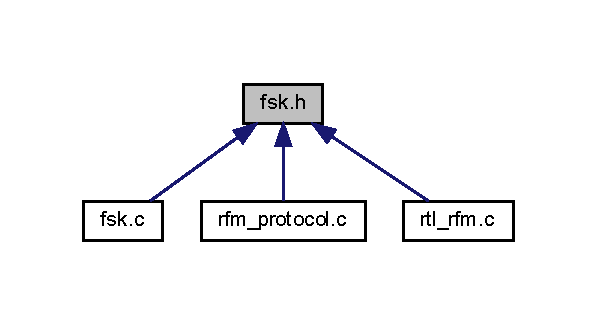
\includegraphics[width=287pt]{fsk_8h__dep__incl}
\end{center}
\end{figure}
\subsection*{Functions}
\begin{DoxyCompactItemize}
\item 
void \hyperlink{fsk_8h_aa5c999a903f4a49095c0acde738ef14e}{fsk\+\_\+init} ()
\item 
void \hyperlink{fsk_8h_a5fc97bcfbea6197fa10974f42cade42c}{fsk\+\_\+cleanup} ()
\item 
int8\+\_\+t \hyperlink{fsk_8h_a7bb9ea952766092f06987bb89d13c60a}{fsk\+\_\+decode} (int16\+\_\+t sample, int16\+\_\+t magnitude)
\end{DoxyCompactItemize}
\subsection*{Variables}
\begin{DoxyCompactItemize}
\item 
int \hyperlink{fsk_8h_ac38751c7169cfeb9325a947cc0484286}{samplerate}
\item 
int16\+\_\+t \hyperlink{fsk_8h_a07ad0fc8154b9241a95d8f6bc0241412}{latestoffset}
\item 
int16\+\_\+t \hyperlink{fsk_8h_a466ad671826b40065c323e1f477d5f2d}{offsethold}
\item 
bool \hyperlink{fsk_8h_af0129e079b57e897edf00f22cc25f3d4}{hold}
\end{DoxyCompactItemize}


\subsection{Function Documentation}
\mbox{\Hypertarget{fsk_8h_a5fc97bcfbea6197fa10974f42cade42c}\label{fsk_8h_a5fc97bcfbea6197fa10974f42cade42c}} 
\index{fsk.\+h@{fsk.\+h}!fsk\+\_\+cleanup@{fsk\+\_\+cleanup}}
\index{fsk\+\_\+cleanup@{fsk\+\_\+cleanup}!fsk.\+h@{fsk.\+h}}
\subsubsection{\texorpdfstring{fsk\+\_\+cleanup()}{fsk\_cleanup()}}
{\footnotesize\ttfamily void fsk\+\_\+cleanup (\begin{DoxyParamCaption}{ }\end{DoxyParamCaption})}

\mbox{\Hypertarget{fsk_8h_a7bb9ea952766092f06987bb89d13c60a}\label{fsk_8h_a7bb9ea952766092f06987bb89d13c60a}} 
\index{fsk.\+h@{fsk.\+h}!fsk\+\_\+decode@{fsk\+\_\+decode}}
\index{fsk\+\_\+decode@{fsk\+\_\+decode}!fsk.\+h@{fsk.\+h}}
\subsubsection{\texorpdfstring{fsk\+\_\+decode()}{fsk\_decode()}}
{\footnotesize\ttfamily int8\+\_\+t fsk\+\_\+decode (\begin{DoxyParamCaption}\item[{int16\+\_\+t}]{sample,  }\item[{int16\+\_\+t}]{magnitude }\end{DoxyParamCaption})}

Here is the call graph for this function\+:
\nopagebreak
\begin{figure}[H]
\begin{center}
\leavevmode
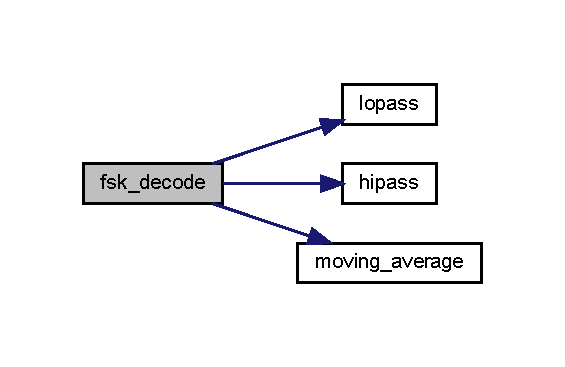
\includegraphics[width=271pt]{fsk_8h_a7bb9ea952766092f06987bb89d13c60a_cgraph}
\end{center}
\end{figure}
\mbox{\Hypertarget{fsk_8h_aa5c999a903f4a49095c0acde738ef14e}\label{fsk_8h_aa5c999a903f4a49095c0acde738ef14e}} 
\index{fsk.\+h@{fsk.\+h}!fsk\+\_\+init@{fsk\+\_\+init}}
\index{fsk\+\_\+init@{fsk\+\_\+init}!fsk.\+h@{fsk.\+h}}
\subsubsection{\texorpdfstring{fsk\+\_\+init()}{fsk\_init()}}
{\footnotesize\ttfamily void fsk\+\_\+init (\begin{DoxyParamCaption}{ }\end{DoxyParamCaption})}

1.\+5; Here is the caller graph for this function\+:
\nopagebreak
\begin{figure}[H]
\begin{center}
\leavevmode
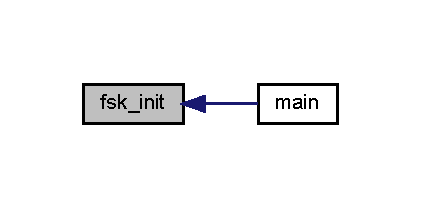
\includegraphics[width=202pt]{fsk_8h_aa5c999a903f4a49095c0acde738ef14e_icgraph}
\end{center}
\end{figure}


\subsection{Variable Documentation}
\mbox{\Hypertarget{fsk_8h_af0129e079b57e897edf00f22cc25f3d4}\label{fsk_8h_af0129e079b57e897edf00f22cc25f3d4}} 
\index{fsk.\+h@{fsk.\+h}!hold@{hold}}
\index{hold@{hold}!fsk.\+h@{fsk.\+h}}
\subsubsection{\texorpdfstring{hold}{hold}}
{\footnotesize\ttfamily bool hold}

\mbox{\Hypertarget{fsk_8h_a07ad0fc8154b9241a95d8f6bc0241412}\label{fsk_8h_a07ad0fc8154b9241a95d8f6bc0241412}} 
\index{fsk.\+h@{fsk.\+h}!latestoffset@{latestoffset}}
\index{latestoffset@{latestoffset}!fsk.\+h@{fsk.\+h}}
\subsubsection{\texorpdfstring{latestoffset}{latestoffset}}
{\footnotesize\ttfamily int16\+\_\+t latestoffset}

\mbox{\Hypertarget{fsk_8h_a466ad671826b40065c323e1f477d5f2d}\label{fsk_8h_a466ad671826b40065c323e1f477d5f2d}} 
\index{fsk.\+h@{fsk.\+h}!offsethold@{offsethold}}
\index{offsethold@{offsethold}!fsk.\+h@{fsk.\+h}}
\subsubsection{\texorpdfstring{offsethold}{offsethold}}
{\footnotesize\ttfamily int16\+\_\+t offsethold}

\mbox{\Hypertarget{fsk_8h_ac38751c7169cfeb9325a947cc0484286}\label{fsk_8h_ac38751c7169cfeb9325a947cc0484286}} 
\index{fsk.\+h@{fsk.\+h}!samplerate@{samplerate}}
\index{samplerate@{samplerate}!fsk.\+h@{fsk.\+h}}
\subsubsection{\texorpdfstring{samplerate}{samplerate}}
{\footnotesize\ttfamily int samplerate}


\hypertarget{_r_e_a_d_m_e_8md}{}\section{R\+E\+A\+D\+M\+E.\+md File Reference}
\label{_r_e_a_d_m_e_8md}\index{R\+E\+A\+D\+M\+E.\+md@{R\+E\+A\+D\+M\+E.\+md}}

\hypertarget{rfm__protocol_8c}{}\section{rfm\+\_\+protocol.\+c File Reference}
\label{rfm__protocol_8c}\index{rfm\+\_\+protocol.\+c@{rfm\+\_\+protocol.\+c}}
{\ttfamily \#include $<$stdio.\+h$>$}\newline
{\ttfamily \#include $<$stdlib.\+h$>$}\newline
{\ttfamily \#include $<$stdbool.\+h$>$}\newline
{\ttfamily \#include $<$stdint.\+h$>$}\newline
{\ttfamily \#include $<$unistd.\+h$>$}\newline
{\ttfamily \#include $<$ctype.\+h$>$}\newline
{\ttfamily \#include $<$string.\+h$>$}\newline
{\ttfamily \#include $<$math.\+h$>$}\newline
{\ttfamily \#include $<$time.\+h$>$}\newline
{\ttfamily \#include \char`\"{}rtl\+\_\+rfm.\+h\char`\"{}}\newline
{\ttfamily \#include \char`\"{}rfm\+\_\+protocol.\+h\char`\"{}}\newline
{\ttfamily \#include \char`\"{}fsk.\+h\char`\"{}}\newline
Include dependency graph for rfm\+\_\+protocol.\+c\+:
\nopagebreak
\begin{figure}[H]
\begin{center}
\leavevmode
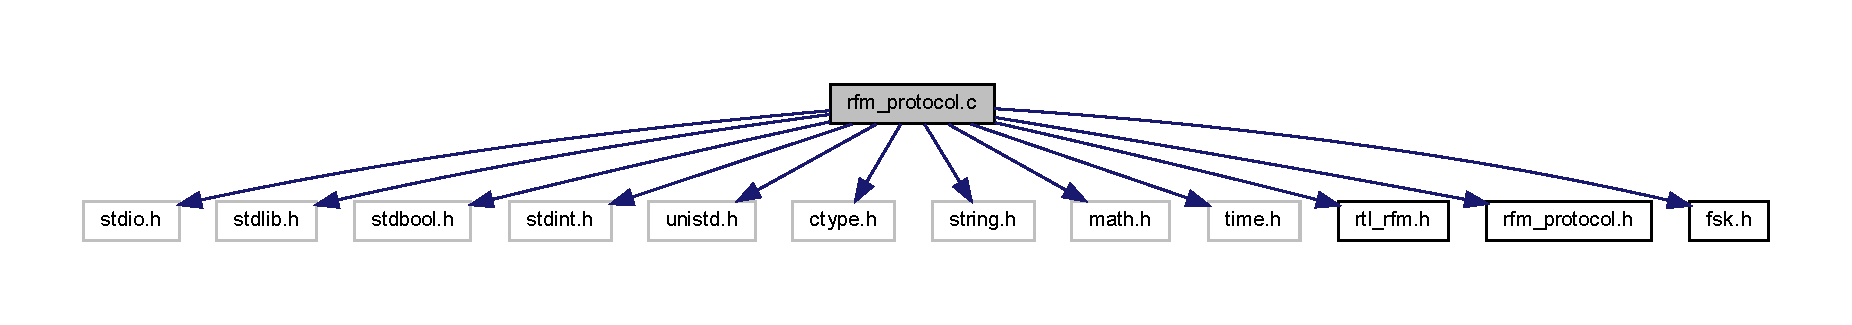
\includegraphics[width=350pt]{rfm__protocol_8c__incl}
\end{center}
\end{figure}
\subsection*{Macros}
\begin{DoxyCompactItemize}
\item 
\#define \hyperlink{rfm__protocol_8c_a67f2b73e9152930dccf1e6d6d48c49f2}{C\+R\+C\+\_\+\+I\+N\+IT}~0x1\+D0F
\item 
\#define \hyperlink{rfm__protocol_8c_a3a57af5c3275b2f53fa64274b11e8d52}{C\+R\+C\+\_\+\+P\+O\+LY}~0x1021
\item 
\#define \hyperlink{rfm__protocol_8c_aebb3fcc0d325b62b5ba320e91cd9fc9c}{C\+R\+C\+\_\+\+P\+O\+ST}~0x\+F\+F\+FF
\end{DoxyCompactItemize}
\subsection*{Functions}
\begin{DoxyCompactItemize}
\item 
void \hyperlink{rfm__protocol_8c_af0ad803b0b174b0e94f2ddd593fa6ed5}{docrc} (uint8\+\_\+t thebyte)
\item 
void \hyperlink{rfm__protocol_8c_a01dd56fff0e704178aa2fbebab398dc5}{print\+\_\+sanitize} (uint8\+\_\+t buf\mbox{[}$\,$\mbox{]}, uint8\+\_\+t \hyperlink{downsampler_8c_a01e8922c4e821da63d9b5060a0a30f45}{bufi})
\item 
void \hyperlink{rfm__protocol_8c_a5bf588658099271d69de7db2203e6c9a}{process\+\_\+byte} (uint8\+\_\+t thebyte)
\item 
void \hyperlink{rfm__protocol_8c_adbfc1cadf9197b8a69a834b2ea57e9d3}{rfm\+\_\+decode} (uint8\+\_\+t thebit)
\end{DoxyCompactItemize}
\subsection*{Variables}
\begin{DoxyCompactItemize}
\item 
int \hyperlink{rfm__protocol_8c_a4ce0852da2ad8307899f6cce4813751e}{bytesexpected} = 0
\item 
int \hyperlink{rfm__protocol_8c_a924c2fd4061ad610b3758afa6e75a1fa}{bitphase} = -\/1
\item 
uint16\+\_\+t \hyperlink{rfm__protocol_8c_aa60093a9a5d5d17864cfda66c47733e3}{crc} = 0x1\+D0F
\item 
uint16\+\_\+t \hyperlink{rfm__protocol_8c_aa1051c12385adb31d013bdc3a5052ce6}{thecrc} = 0
\item 
uint8\+\_\+t \hyperlink{rfm__protocol_8c_ac0ec4addf7c2312ed9b463c5e85578dd}{packet\+\_\+buffer} \mbox{[}256\mbox{]}
\item 
uint8\+\_\+t \hyperlink{rfm__protocol_8c_a1718207ef770c65a305151abf2e32987}{packet\+\_\+bi} = 0
\end{DoxyCompactItemize}


\subsection{Macro Definition Documentation}
\mbox{\Hypertarget{rfm__protocol_8c_a67f2b73e9152930dccf1e6d6d48c49f2}\label{rfm__protocol_8c_a67f2b73e9152930dccf1e6d6d48c49f2}} 
\index{rfm\+\_\+protocol.\+c@{rfm\+\_\+protocol.\+c}!C\+R\+C\+\_\+\+I\+N\+IT@{C\+R\+C\+\_\+\+I\+N\+IT}}
\index{C\+R\+C\+\_\+\+I\+N\+IT@{C\+R\+C\+\_\+\+I\+N\+IT}!rfm\+\_\+protocol.\+c@{rfm\+\_\+protocol.\+c}}
\subsubsection{\texorpdfstring{C\+R\+C\+\_\+\+I\+N\+IT}{CRC\_INIT}}
{\footnotesize\ttfamily \#define C\+R\+C\+\_\+\+I\+N\+IT~0x1\+D0F}

\mbox{\Hypertarget{rfm__protocol_8c_a3a57af5c3275b2f53fa64274b11e8d52}\label{rfm__protocol_8c_a3a57af5c3275b2f53fa64274b11e8d52}} 
\index{rfm\+\_\+protocol.\+c@{rfm\+\_\+protocol.\+c}!C\+R\+C\+\_\+\+P\+O\+LY@{C\+R\+C\+\_\+\+P\+O\+LY}}
\index{C\+R\+C\+\_\+\+P\+O\+LY@{C\+R\+C\+\_\+\+P\+O\+LY}!rfm\+\_\+protocol.\+c@{rfm\+\_\+protocol.\+c}}
\subsubsection{\texorpdfstring{C\+R\+C\+\_\+\+P\+O\+LY}{CRC\_POLY}}
{\footnotesize\ttfamily \#define C\+R\+C\+\_\+\+P\+O\+LY~0x1021}

\mbox{\Hypertarget{rfm__protocol_8c_aebb3fcc0d325b62b5ba320e91cd9fc9c}\label{rfm__protocol_8c_aebb3fcc0d325b62b5ba320e91cd9fc9c}} 
\index{rfm\+\_\+protocol.\+c@{rfm\+\_\+protocol.\+c}!C\+R\+C\+\_\+\+P\+O\+ST@{C\+R\+C\+\_\+\+P\+O\+ST}}
\index{C\+R\+C\+\_\+\+P\+O\+ST@{C\+R\+C\+\_\+\+P\+O\+ST}!rfm\+\_\+protocol.\+c@{rfm\+\_\+protocol.\+c}}
\subsubsection{\texorpdfstring{C\+R\+C\+\_\+\+P\+O\+ST}{CRC\_POST}}
{\footnotesize\ttfamily \#define C\+R\+C\+\_\+\+P\+O\+ST~0x\+F\+F\+FF}



\subsection{Function Documentation}
\mbox{\Hypertarget{rfm__protocol_8c_af0ad803b0b174b0e94f2ddd593fa6ed5}\label{rfm__protocol_8c_af0ad803b0b174b0e94f2ddd593fa6ed5}} 
\index{rfm\+\_\+protocol.\+c@{rfm\+\_\+protocol.\+c}!docrc@{docrc}}
\index{docrc@{docrc}!rfm\+\_\+protocol.\+c@{rfm\+\_\+protocol.\+c}}
\subsubsection{\texorpdfstring{docrc()}{docrc()}}
{\footnotesize\ttfamily void docrc (\begin{DoxyParamCaption}\item[{uint8\+\_\+t}]{thebyte }\end{DoxyParamCaption})}

Here is the caller graph for this function\+:
\nopagebreak
\begin{figure}[H]
\begin{center}
\leavevmode
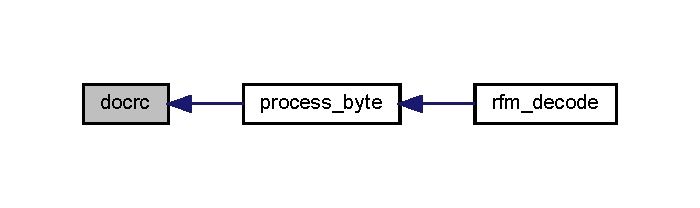
\includegraphics[width=336pt]{rfm__protocol_8c_af0ad803b0b174b0e94f2ddd593fa6ed5_icgraph}
\end{center}
\end{figure}
\mbox{\Hypertarget{rfm__protocol_8c_a01dd56fff0e704178aa2fbebab398dc5}\label{rfm__protocol_8c_a01dd56fff0e704178aa2fbebab398dc5}} 
\index{rfm\+\_\+protocol.\+c@{rfm\+\_\+protocol.\+c}!print\+\_\+sanitize@{print\+\_\+sanitize}}
\index{print\+\_\+sanitize@{print\+\_\+sanitize}!rfm\+\_\+protocol.\+c@{rfm\+\_\+protocol.\+c}}
\subsubsection{\texorpdfstring{print\+\_\+sanitize()}{print\_sanitize()}}
{\footnotesize\ttfamily void print\+\_\+sanitize (\begin{DoxyParamCaption}\item[{uint8\+\_\+t}]{buf\mbox{[}$\,$\mbox{]},  }\item[{uint8\+\_\+t}]{bufi }\end{DoxyParamCaption})}

Here is the caller graph for this function\+:
\nopagebreak
\begin{figure}[H]
\begin{center}
\leavevmode
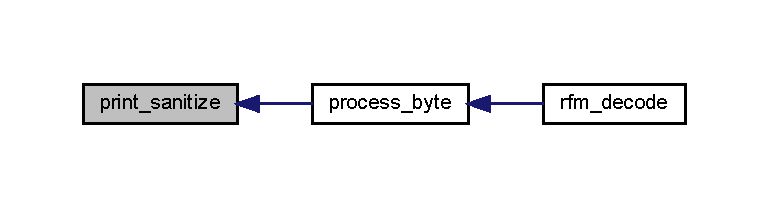
\includegraphics[width=350pt]{rfm__protocol_8c_a01dd56fff0e704178aa2fbebab398dc5_icgraph}
\end{center}
\end{figure}
\mbox{\Hypertarget{rfm__protocol_8c_a5bf588658099271d69de7db2203e6c9a}\label{rfm__protocol_8c_a5bf588658099271d69de7db2203e6c9a}} 
\index{rfm\+\_\+protocol.\+c@{rfm\+\_\+protocol.\+c}!process\+\_\+byte@{process\+\_\+byte}}
\index{process\+\_\+byte@{process\+\_\+byte}!rfm\+\_\+protocol.\+c@{rfm\+\_\+protocol.\+c}}
\subsubsection{\texorpdfstring{process\+\_\+byte()}{process\_byte()}}
{\footnotesize\ttfamily void process\+\_\+byte (\begin{DoxyParamCaption}\item[{uint8\+\_\+t}]{thebyte }\end{DoxyParamCaption})}

Here is the call graph for this function\+:
\nopagebreak
\begin{figure}[H]
\begin{center}
\leavevmode
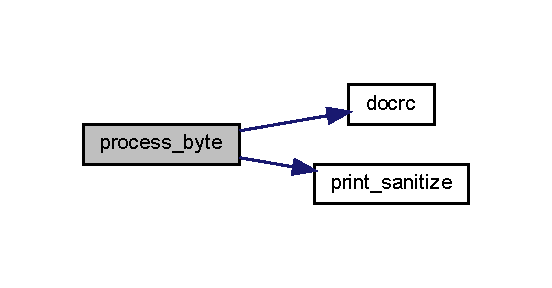
\includegraphics[width=265pt]{rfm__protocol_8c_a5bf588658099271d69de7db2203e6c9a_cgraph}
\end{center}
\end{figure}
Here is the caller graph for this function\+:
\nopagebreak
\begin{figure}[H]
\begin{center}
\leavevmode
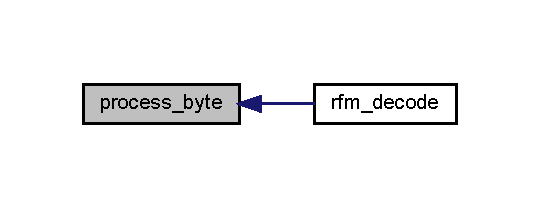
\includegraphics[width=259pt]{rfm__protocol_8c_a5bf588658099271d69de7db2203e6c9a_icgraph}
\end{center}
\end{figure}
\mbox{\Hypertarget{rfm__protocol_8c_adbfc1cadf9197b8a69a834b2ea57e9d3}\label{rfm__protocol_8c_adbfc1cadf9197b8a69a834b2ea57e9d3}} 
\index{rfm\+\_\+protocol.\+c@{rfm\+\_\+protocol.\+c}!rfm\+\_\+decode@{rfm\+\_\+decode}}
\index{rfm\+\_\+decode@{rfm\+\_\+decode}!rfm\+\_\+protocol.\+c@{rfm\+\_\+protocol.\+c}}
\subsubsection{\texorpdfstring{rfm\+\_\+decode()}{rfm\_decode()}}
{\footnotesize\ttfamily void rfm\+\_\+decode (\begin{DoxyParamCaption}\item[{uint8\+\_\+t}]{thebit }\end{DoxyParamCaption})}

Here is the call graph for this function\+:
\nopagebreak
\begin{figure}[H]
\begin{center}
\leavevmode
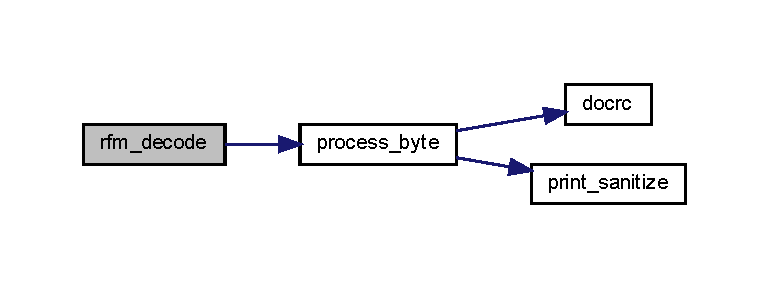
\includegraphics[width=350pt]{rfm__protocol_8c_adbfc1cadf9197b8a69a834b2ea57e9d3_cgraph}
\end{center}
\end{figure}


\subsection{Variable Documentation}
\mbox{\Hypertarget{rfm__protocol_8c_a924c2fd4061ad610b3758afa6e75a1fa}\label{rfm__protocol_8c_a924c2fd4061ad610b3758afa6e75a1fa}} 
\index{rfm\+\_\+protocol.\+c@{rfm\+\_\+protocol.\+c}!bitphase@{bitphase}}
\index{bitphase@{bitphase}!rfm\+\_\+protocol.\+c@{rfm\+\_\+protocol.\+c}}
\subsubsection{\texorpdfstring{bitphase}{bitphase}}
{\footnotesize\ttfamily int bitphase = -\/1}

\mbox{\Hypertarget{rfm__protocol_8c_a4ce0852da2ad8307899f6cce4813751e}\label{rfm__protocol_8c_a4ce0852da2ad8307899f6cce4813751e}} 
\index{rfm\+\_\+protocol.\+c@{rfm\+\_\+protocol.\+c}!bytesexpected@{bytesexpected}}
\index{bytesexpected@{bytesexpected}!rfm\+\_\+protocol.\+c@{rfm\+\_\+protocol.\+c}}
\subsubsection{\texorpdfstring{bytesexpected}{bytesexpected}}
{\footnotesize\ttfamily int bytesexpected = 0}

\mbox{\Hypertarget{rfm__protocol_8c_aa60093a9a5d5d17864cfda66c47733e3}\label{rfm__protocol_8c_aa60093a9a5d5d17864cfda66c47733e3}} 
\index{rfm\+\_\+protocol.\+c@{rfm\+\_\+protocol.\+c}!crc@{crc}}
\index{crc@{crc}!rfm\+\_\+protocol.\+c@{rfm\+\_\+protocol.\+c}}
\subsubsection{\texorpdfstring{crc}{crc}}
{\footnotesize\ttfamily uint16\+\_\+t crc = 0x1\+D0F}

\mbox{\Hypertarget{rfm__protocol_8c_a1718207ef770c65a305151abf2e32987}\label{rfm__protocol_8c_a1718207ef770c65a305151abf2e32987}} 
\index{rfm\+\_\+protocol.\+c@{rfm\+\_\+protocol.\+c}!packet\+\_\+bi@{packet\+\_\+bi}}
\index{packet\+\_\+bi@{packet\+\_\+bi}!rfm\+\_\+protocol.\+c@{rfm\+\_\+protocol.\+c}}
\subsubsection{\texorpdfstring{packet\+\_\+bi}{packet\_bi}}
{\footnotesize\ttfamily uint8\+\_\+t packet\+\_\+bi = 0}

\mbox{\Hypertarget{rfm__protocol_8c_ac0ec4addf7c2312ed9b463c5e85578dd}\label{rfm__protocol_8c_ac0ec4addf7c2312ed9b463c5e85578dd}} 
\index{rfm\+\_\+protocol.\+c@{rfm\+\_\+protocol.\+c}!packet\+\_\+buffer@{packet\+\_\+buffer}}
\index{packet\+\_\+buffer@{packet\+\_\+buffer}!rfm\+\_\+protocol.\+c@{rfm\+\_\+protocol.\+c}}
\subsubsection{\texorpdfstring{packet\+\_\+buffer}{packet\_buffer}}
{\footnotesize\ttfamily uint8\+\_\+t packet\+\_\+buffer\mbox{[}256\mbox{]}}

\mbox{\Hypertarget{rfm__protocol_8c_aa1051c12385adb31d013bdc3a5052ce6}\label{rfm__protocol_8c_aa1051c12385adb31d013bdc3a5052ce6}} 
\index{rfm\+\_\+protocol.\+c@{rfm\+\_\+protocol.\+c}!thecrc@{thecrc}}
\index{thecrc@{thecrc}!rfm\+\_\+protocol.\+c@{rfm\+\_\+protocol.\+c}}
\subsubsection{\texorpdfstring{thecrc}{thecrc}}
{\footnotesize\ttfamily uint16\+\_\+t thecrc = 0}


\hypertarget{rfm__protocol_8h}{}\section{rfm\+\_\+protocol.\+h File Reference}
\label{rfm__protocol_8h}\index{rfm\+\_\+protocol.\+h@{rfm\+\_\+protocol.\+h}}
This graph shows which files directly or indirectly include this file\+:
\nopagebreak
\begin{figure}[H]
\begin{center}
\leavevmode
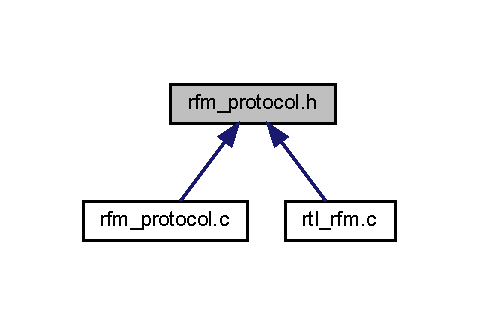
\includegraphics[width=230pt]{rfm__protocol_8h__dep__incl}
\end{center}
\end{figure}
\subsection*{Functions}
\begin{DoxyCompactItemize}
\item 
void \hyperlink{rfm__protocol_8h_adbfc1cadf9197b8a69a834b2ea57e9d3}{rfm\+\_\+decode} (uint8\+\_\+t thebit)
\end{DoxyCompactItemize}


\subsection{Function Documentation}
\mbox{\Hypertarget{rfm__protocol_8h_adbfc1cadf9197b8a69a834b2ea57e9d3}\label{rfm__protocol_8h_adbfc1cadf9197b8a69a834b2ea57e9d3}} 
\index{rfm\+\_\+protocol.\+h@{rfm\+\_\+protocol.\+h}!rfm\+\_\+decode@{rfm\+\_\+decode}}
\index{rfm\+\_\+decode@{rfm\+\_\+decode}!rfm\+\_\+protocol.\+h@{rfm\+\_\+protocol.\+h}}
\subsubsection{\texorpdfstring{rfm\+\_\+decode()}{rfm\_decode()}}
{\footnotesize\ttfamily void rfm\+\_\+decode (\begin{DoxyParamCaption}\item[{uint8\+\_\+t}]{thebit }\end{DoxyParamCaption})}

Here is the call graph for this function\+:
\nopagebreak
\begin{figure}[H]
\begin{center}
\leavevmode
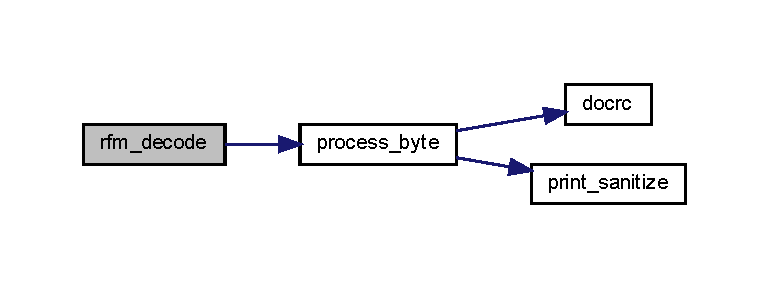
\includegraphics[width=350pt]{rfm__protocol_8h_adbfc1cadf9197b8a69a834b2ea57e9d3_cgraph}
\end{center}
\end{figure}

\hypertarget{rtl__rfm_8c}{}\section{rtl\+\_\+rfm.\+c File Reference}
\label{rtl__rfm_8c}\index{rtl\+\_\+rfm.\+c@{rtl\+\_\+rfm.\+c}}
{\ttfamily \#include $<$stdio.\+h$>$}\newline
{\ttfamily \#include $<$stdlib.\+h$>$}\newline
{\ttfamily \#include $<$stdbool.\+h$>$}\newline
{\ttfamily \#include $<$stdint.\+h$>$}\newline
{\ttfamily \#include $<$unistd.\+h$>$}\newline
{\ttfamily \#include $<$ctype.\+h$>$}\newline
{\ttfamily \#include $<$string.\+h$>$}\newline
{\ttfamily \#include $<$math.\+h$>$}\newline
{\ttfamily \#include $<$time.\+h$>$}\newline
{\ttfamily \#include $<$signal.\+h$>$}\newline
{\ttfamily \#include $<$errno.\+h$>$}\newline
{\ttfamily \#include \char`\"{}rtl\+\_\+rfm.\+h\char`\"{}}\newline
{\ttfamily \#include \char`\"{}downsampler.\+h\char`\"{}}\newline
{\ttfamily \#include \char`\"{}fm.\+h\char`\"{}}\newline
{\ttfamily \#include \char`\"{}fsk.\+h\char`\"{}}\newline
{\ttfamily \#include \char`\"{}rfm\+\_\+protocol.\+h\char`\"{}}\newline
Include dependency graph for rtl\+\_\+rfm.\+c\+:
\nopagebreak
\begin{figure}[H]
\begin{center}
\leavevmode
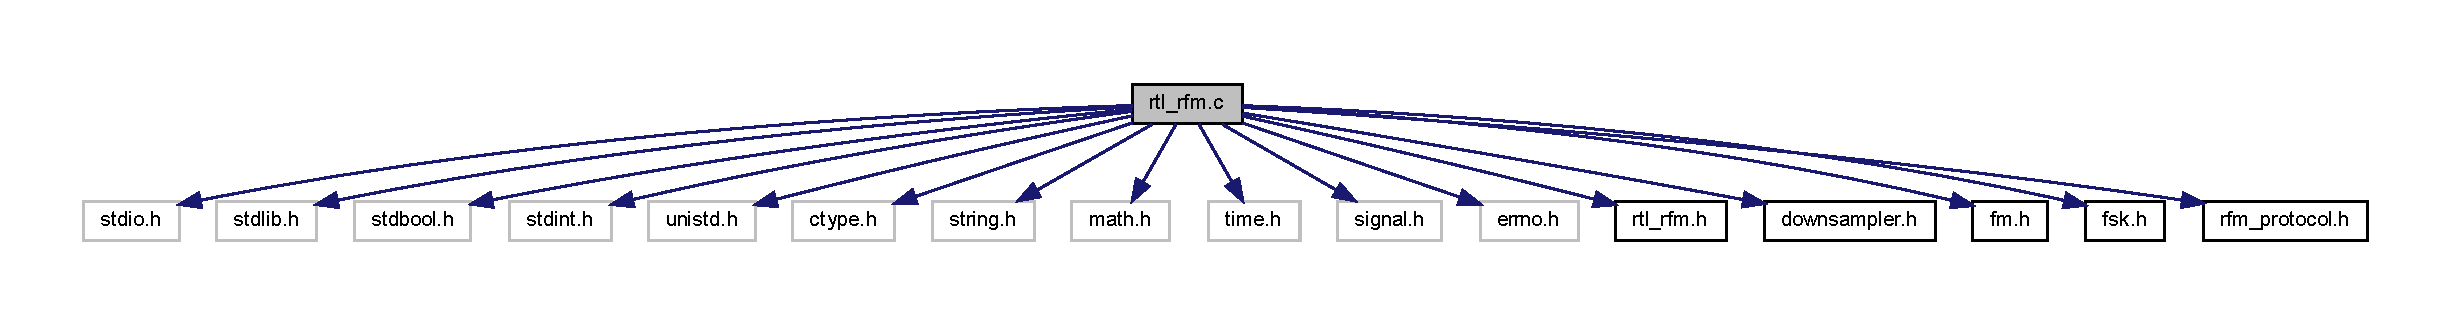
\includegraphics[width=350pt]{rtl__rfm_8c__incl}
\end{center}
\end{figure}
\subsection*{Functions}
\begin{DoxyCompactItemize}
\item 
void \hyperlink{rtl__rfm_8c_a3b33e6f48f5d988f336e915c5346eb95}{int\+Handler} (int dummy)
\item 
int \hyperlink{rtl__rfm_8c_a3c04138a5bfe5d72780bb7e82a18e627}{main} (int argc, char $\ast$$\ast$argv)
\end{DoxyCompactItemize}
\subsection*{Variables}
\begin{DoxyCompactItemize}
\item 
int \hyperlink{rtl__rfm_8c_ad65a8842cc674e3ddf69355898c0ecbf}{errno}
\item 
bool \hyperlink{rtl__rfm_8c_ae4426f467d61ae456b95844d4d9c2dcd}{quiet} = false
\item 
bool \hyperlink{rtl__rfm_8c_a228850c9a9875ce019a8e06ec23b4c50}{debugplot} = false
\item 
int \hyperlink{rtl__rfm_8c_ae0d22272b68e75d19ac0b80c01f806b6}{freq} = 869412500
\item 
int \hyperlink{rtl__rfm_8c_ad209a6b4e081cf7b984dcfe8ceb7c50d}{gain} = 50
\item 
int \hyperlink{rtl__rfm_8c_adfa704ac0ad5feeb79d94c9c9119f7ec}{ppm} = 43
\item 
int \hyperlink{rtl__rfm_8c_acc64b53c6036b7b11d4ae688994f0b56}{baudrate} = 4800
\item 
F\+I\+LE $\ast$ \hyperlink{rtl__rfm_8c_a2def6792e5a0f01335f7cdcf839d5fee}{rtlstream} = N\+U\+LL
\end{DoxyCompactItemize}


\subsection{Function Documentation}
\mbox{\Hypertarget{rtl__rfm_8c_a3b33e6f48f5d988f336e915c5346eb95}\label{rtl__rfm_8c_a3b33e6f48f5d988f336e915c5346eb95}} 
\index{rtl\+\_\+rfm.\+c@{rtl\+\_\+rfm.\+c}!int\+Handler@{int\+Handler}}
\index{int\+Handler@{int\+Handler}!rtl\+\_\+rfm.\+c@{rtl\+\_\+rfm.\+c}}
\subsubsection{\texorpdfstring{int\+Handler()}{intHandler()}}
{\footnotesize\ttfamily void int\+Handler (\begin{DoxyParamCaption}\item[{int}]{dummy }\end{DoxyParamCaption})}

Here is the caller graph for this function\+:
\nopagebreak
\begin{figure}[H]
\begin{center}
\leavevmode
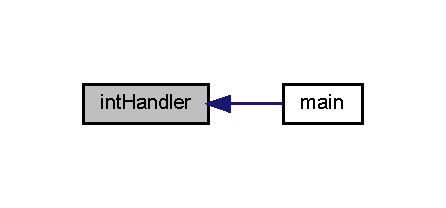
\includegraphics[width=214pt]{rtl__rfm_8c_a3b33e6f48f5d988f336e915c5346eb95_icgraph}
\end{center}
\end{figure}
\mbox{\Hypertarget{rtl__rfm_8c_a3c04138a5bfe5d72780bb7e82a18e627}\label{rtl__rfm_8c_a3c04138a5bfe5d72780bb7e82a18e627}} 
\index{rtl\+\_\+rfm.\+c@{rtl\+\_\+rfm.\+c}!main@{main}}
\index{main@{main}!rtl\+\_\+rfm.\+c@{rtl\+\_\+rfm.\+c}}
\subsubsection{\texorpdfstring{main()}{main()}}
{\footnotesize\ttfamily int main (\begin{DoxyParamCaption}\item[{int}]{argc,  }\item[{char $\ast$$\ast$}]{argv }\end{DoxyParamCaption})}

Here is the call graph for this function\+:
\nopagebreak
\begin{figure}[H]
\begin{center}
\leavevmode
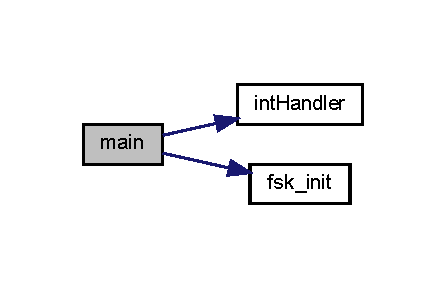
\includegraphics[width=214pt]{rtl__rfm_8c_a3c04138a5bfe5d72780bb7e82a18e627_cgraph}
\end{center}
\end{figure}


\subsection{Variable Documentation}
\mbox{\Hypertarget{rtl__rfm_8c_acc64b53c6036b7b11d4ae688994f0b56}\label{rtl__rfm_8c_acc64b53c6036b7b11d4ae688994f0b56}} 
\index{rtl\+\_\+rfm.\+c@{rtl\+\_\+rfm.\+c}!baudrate@{baudrate}}
\index{baudrate@{baudrate}!rtl\+\_\+rfm.\+c@{rtl\+\_\+rfm.\+c}}
\subsubsection{\texorpdfstring{baudrate}{baudrate}}
{\footnotesize\ttfamily int baudrate = 4800}

\mbox{\Hypertarget{rtl__rfm_8c_a228850c9a9875ce019a8e06ec23b4c50}\label{rtl__rfm_8c_a228850c9a9875ce019a8e06ec23b4c50}} 
\index{rtl\+\_\+rfm.\+c@{rtl\+\_\+rfm.\+c}!debugplot@{debugplot}}
\index{debugplot@{debugplot}!rtl\+\_\+rfm.\+c@{rtl\+\_\+rfm.\+c}}
\subsubsection{\texorpdfstring{debugplot}{debugplot}}
{\footnotesize\ttfamily bool debugplot = false}

\mbox{\Hypertarget{rtl__rfm_8c_ad65a8842cc674e3ddf69355898c0ecbf}\label{rtl__rfm_8c_ad65a8842cc674e3ddf69355898c0ecbf}} 
\index{rtl\+\_\+rfm.\+c@{rtl\+\_\+rfm.\+c}!errno@{errno}}
\index{errno@{errno}!rtl\+\_\+rfm.\+c@{rtl\+\_\+rfm.\+c}}
\subsubsection{\texorpdfstring{errno}{errno}}
{\footnotesize\ttfamily int errno}

\mbox{\Hypertarget{rtl__rfm_8c_ae0d22272b68e75d19ac0b80c01f806b6}\label{rtl__rfm_8c_ae0d22272b68e75d19ac0b80c01f806b6}} 
\index{rtl\+\_\+rfm.\+c@{rtl\+\_\+rfm.\+c}!freq@{freq}}
\index{freq@{freq}!rtl\+\_\+rfm.\+c@{rtl\+\_\+rfm.\+c}}
\subsubsection{\texorpdfstring{freq}{freq}}
{\footnotesize\ttfamily int freq = 869412500}

\mbox{\Hypertarget{rtl__rfm_8c_ad209a6b4e081cf7b984dcfe8ceb7c50d}\label{rtl__rfm_8c_ad209a6b4e081cf7b984dcfe8ceb7c50d}} 
\index{rtl\+\_\+rfm.\+c@{rtl\+\_\+rfm.\+c}!gain@{gain}}
\index{gain@{gain}!rtl\+\_\+rfm.\+c@{rtl\+\_\+rfm.\+c}}
\subsubsection{\texorpdfstring{gain}{gain}}
{\footnotesize\ttfamily int gain = 50}

\mbox{\Hypertarget{rtl__rfm_8c_adfa704ac0ad5feeb79d94c9c9119f7ec}\label{rtl__rfm_8c_adfa704ac0ad5feeb79d94c9c9119f7ec}} 
\index{rtl\+\_\+rfm.\+c@{rtl\+\_\+rfm.\+c}!ppm@{ppm}}
\index{ppm@{ppm}!rtl\+\_\+rfm.\+c@{rtl\+\_\+rfm.\+c}}
\subsubsection{\texorpdfstring{ppm}{ppm}}
{\footnotesize\ttfamily int ppm = 43}

\mbox{\Hypertarget{rtl__rfm_8c_ae4426f467d61ae456b95844d4d9c2dcd}\label{rtl__rfm_8c_ae4426f467d61ae456b95844d4d9c2dcd}} 
\index{rtl\+\_\+rfm.\+c@{rtl\+\_\+rfm.\+c}!quiet@{quiet}}
\index{quiet@{quiet}!rtl\+\_\+rfm.\+c@{rtl\+\_\+rfm.\+c}}
\subsubsection{\texorpdfstring{quiet}{quiet}}
{\footnotesize\ttfamily bool quiet = false}

\mbox{\Hypertarget{rtl__rfm_8c_a2def6792e5a0f01335f7cdcf839d5fee}\label{rtl__rfm_8c_a2def6792e5a0f01335f7cdcf839d5fee}} 
\index{rtl\+\_\+rfm.\+c@{rtl\+\_\+rfm.\+c}!rtlstream@{rtlstream}}
\index{rtlstream@{rtlstream}!rtl\+\_\+rfm.\+c@{rtl\+\_\+rfm.\+c}}
\subsubsection{\texorpdfstring{rtlstream}{rtlstream}}
{\footnotesize\ttfamily F\+I\+LE$\ast$ rtlstream = N\+U\+LL}


\hypertarget{rtl__rfm_8h}{}\section{rtl\+\_\+rfm.\+h File Reference}
\label{rtl__rfm_8h}\index{rtl\+\_\+rfm.\+h@{rtl\+\_\+rfm.\+h}}
This graph shows which files directly or indirectly include this file\+:
\nopagebreak
\begin{figure}[H]
\begin{center}
\leavevmode
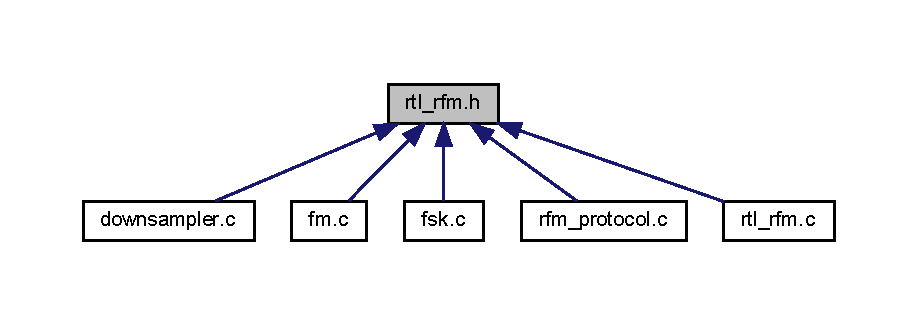
\includegraphics[width=350pt]{rtl__rfm_8h__dep__incl}
\end{center}
\end{figure}
\subsection*{Macros}
\begin{DoxyCompactItemize}
\item 
\#define \hyperlink{rtl__rfm_8h_a81ab58068676f17bd9788a2e01dac6d3}{B\+I\+G\+S\+A\+M\+P\+L\+E\+R\+A\+TE}~2457600
\item 
\#define \hyperlink{rtl__rfm_8h_a061e870517c5d5c01d232d72e5b6857f}{D\+O\+W\+N\+S\+A\+M\+P\+LE}~64
\end{DoxyCompactItemize}
\subsection*{Variables}
\begin{DoxyCompactItemize}
\item 
bool \hyperlink{rtl__rfm_8h_ae4426f467d61ae456b95844d4d9c2dcd}{quiet}
\item 
bool \hyperlink{rtl__rfm_8h_a228850c9a9875ce019a8e06ec23b4c50}{debugplot}
\item 
int \hyperlink{rtl__rfm_8h_ae0d22272b68e75d19ac0b80c01f806b6}{freq}
\item 
int \hyperlink{rtl__rfm_8h_ad209a6b4e081cf7b984dcfe8ceb7c50d}{gain}
\item 
int \hyperlink{rtl__rfm_8h_adfa704ac0ad5feeb79d94c9c9119f7ec}{ppm}
\item 
int \hyperlink{rtl__rfm_8h_acc64b53c6036b7b11d4ae688994f0b56}{baudrate}
\end{DoxyCompactItemize}


\subsection{Macro Definition Documentation}
\mbox{\Hypertarget{rtl__rfm_8h_a81ab58068676f17bd9788a2e01dac6d3}\label{rtl__rfm_8h_a81ab58068676f17bd9788a2e01dac6d3}} 
\index{rtl\+\_\+rfm.\+h@{rtl\+\_\+rfm.\+h}!B\+I\+G\+S\+A\+M\+P\+L\+E\+R\+A\+TE@{B\+I\+G\+S\+A\+M\+P\+L\+E\+R\+A\+TE}}
\index{B\+I\+G\+S\+A\+M\+P\+L\+E\+R\+A\+TE@{B\+I\+G\+S\+A\+M\+P\+L\+E\+R\+A\+TE}!rtl\+\_\+rfm.\+h@{rtl\+\_\+rfm.\+h}}
\subsubsection{\texorpdfstring{B\+I\+G\+S\+A\+M\+P\+L\+E\+R\+A\+TE}{BIGSAMPLERATE}}
{\footnotesize\ttfamily \#define B\+I\+G\+S\+A\+M\+P\+L\+E\+R\+A\+TE~2457600}

\mbox{\Hypertarget{rtl__rfm_8h_a061e870517c5d5c01d232d72e5b6857f}\label{rtl__rfm_8h_a061e870517c5d5c01d232d72e5b6857f}} 
\index{rtl\+\_\+rfm.\+h@{rtl\+\_\+rfm.\+h}!D\+O\+W\+N\+S\+A\+M\+P\+LE@{D\+O\+W\+N\+S\+A\+M\+P\+LE}}
\index{D\+O\+W\+N\+S\+A\+M\+P\+LE@{D\+O\+W\+N\+S\+A\+M\+P\+LE}!rtl\+\_\+rfm.\+h@{rtl\+\_\+rfm.\+h}}
\subsubsection{\texorpdfstring{D\+O\+W\+N\+S\+A\+M\+P\+LE}{DOWNSAMPLE}}
{\footnotesize\ttfamily \#define D\+O\+W\+N\+S\+A\+M\+P\+LE~64}



\subsection{Variable Documentation}
\mbox{\Hypertarget{rtl__rfm_8h_acc64b53c6036b7b11d4ae688994f0b56}\label{rtl__rfm_8h_acc64b53c6036b7b11d4ae688994f0b56}} 
\index{rtl\+\_\+rfm.\+h@{rtl\+\_\+rfm.\+h}!baudrate@{baudrate}}
\index{baudrate@{baudrate}!rtl\+\_\+rfm.\+h@{rtl\+\_\+rfm.\+h}}
\subsubsection{\texorpdfstring{baudrate}{baudrate}}
{\footnotesize\ttfamily int baudrate}

\mbox{\Hypertarget{rtl__rfm_8h_a228850c9a9875ce019a8e06ec23b4c50}\label{rtl__rfm_8h_a228850c9a9875ce019a8e06ec23b4c50}} 
\index{rtl\+\_\+rfm.\+h@{rtl\+\_\+rfm.\+h}!debugplot@{debugplot}}
\index{debugplot@{debugplot}!rtl\+\_\+rfm.\+h@{rtl\+\_\+rfm.\+h}}
\subsubsection{\texorpdfstring{debugplot}{debugplot}}
{\footnotesize\ttfamily bool debugplot}

\mbox{\Hypertarget{rtl__rfm_8h_ae0d22272b68e75d19ac0b80c01f806b6}\label{rtl__rfm_8h_ae0d22272b68e75d19ac0b80c01f806b6}} 
\index{rtl\+\_\+rfm.\+h@{rtl\+\_\+rfm.\+h}!freq@{freq}}
\index{freq@{freq}!rtl\+\_\+rfm.\+h@{rtl\+\_\+rfm.\+h}}
\subsubsection{\texorpdfstring{freq}{freq}}
{\footnotesize\ttfamily int freq}

\mbox{\Hypertarget{rtl__rfm_8h_ad209a6b4e081cf7b984dcfe8ceb7c50d}\label{rtl__rfm_8h_ad209a6b4e081cf7b984dcfe8ceb7c50d}} 
\index{rtl\+\_\+rfm.\+h@{rtl\+\_\+rfm.\+h}!gain@{gain}}
\index{gain@{gain}!rtl\+\_\+rfm.\+h@{rtl\+\_\+rfm.\+h}}
\subsubsection{\texorpdfstring{gain}{gain}}
{\footnotesize\ttfamily int gain}

\mbox{\Hypertarget{rtl__rfm_8h_adfa704ac0ad5feeb79d94c9c9119f7ec}\label{rtl__rfm_8h_adfa704ac0ad5feeb79d94c9c9119f7ec}} 
\index{rtl\+\_\+rfm.\+h@{rtl\+\_\+rfm.\+h}!ppm@{ppm}}
\index{ppm@{ppm}!rtl\+\_\+rfm.\+h@{rtl\+\_\+rfm.\+h}}
\subsubsection{\texorpdfstring{ppm}{ppm}}
{\footnotesize\ttfamily int ppm}

\mbox{\Hypertarget{rtl__rfm_8h_ae4426f467d61ae456b95844d4d9c2dcd}\label{rtl__rfm_8h_ae4426f467d61ae456b95844d4d9c2dcd}} 
\index{rtl\+\_\+rfm.\+h@{rtl\+\_\+rfm.\+h}!quiet@{quiet}}
\index{quiet@{quiet}!rtl\+\_\+rfm.\+h@{rtl\+\_\+rfm.\+h}}
\subsubsection{\texorpdfstring{quiet}{quiet}}
{\footnotesize\ttfamily bool quiet}


%--- End generated contents ---

% Index
\backmatter
\newpage
\phantomsection
\clearemptydoublepage
\addcontentsline{toc}{chapter}{Index}
\printindex

\end{document}
